% Tệp mẫu làm đề thi trắc nghiệm dựa vào gói lệnh dethi.sty 3.2
% Tác giả: Nguyên Hữu Điển
% Khoa Toán Cơ Tin học, ĐHKHTN HN, ĐHQGHN
% 334, Nguyễn Trãi, Thanh Xuân, Hà Nội
% huudien@vnu.edu.vn
% Ngày 26/12/2009
%%%%%%%%%%%%%%%%%%%%%%%%%%%%
\documentclass[11pt,openany]{article}
\usepackage{amsmath,amsxtra,amssymb,latexsym, amscd,amsthm}
\usepackage{graphicx}
\usepackage{picinpar}
\usepackage{tikz}
\usetikzlibrary{arrows}
\usepackage{tkz-tab}
\usepackage[utf8]{vietnam}
\usepackage{longtable}%
\usepackage{multicol}%
\usepackage{color}
 \usepackage{shortlst}
\usepackage{mathpazo} 
\usepackage[bookmarksnumbered, colorlinks,hyperindex, unicode]{hyperref}%
\usepackage{titledot}
\voffset=-2cm
% \hoffset=-2cm
\textheight 24truecm 
\textwidth 18truecm 
\usepackage[baitap]{dethi}
\usepackage{fancyhdr}
\pagestyle{fancy}
\renewcommand{\sectionmark}[1]%
           {\markright{\it \thesection\ #1}}
\lhead[\fancyplain{}{
     \footnotesize{Page \thepage\ of \pageref{LastPage}}}]
{\fancyplain{}{ https://nhdien.wordpress.com - {\it Nguyễn Hữu Điển}}}
\rhead[\fancyplain{}{\leftmark}]%
   {\fancyplain{}{\footnotesize{Trang số \thepage\ trong \pageref{LastPage}}}}
\cfoot{\footnotesize{\thepage/\pageref{LastPage}}}
\sloppy

\tentruong{ĐẠI HỌC KHOA HỌC TỰ NHIÊN}
\tenkhoa{Khoa Toán - Cơ -Tin học}
\loaidethi{Đề gồm có \pageref{LastPage} trang}
\tenkythi{ĐỀ THI GIỮA KỲ NĂM HỌC 2016-2017}
\tenmonhoc{Môn: Toán học tính toán}
\madethi{100}
\thoigian{\underline{Thời gian làm bài: 90 phút, không kể thời gian phát đề}}   
\hovaten{Họ và tên}         %Nếu không muốn có dòng này không gõ lệnh
\tenlop{Tên lớp}         %Nếu không muốn có dòng này không gõ lệnh
\sobaodanh{Số báo danh}  %Nếu không muốn có dòng này không gõ lệnh

\usepackage{fancybox}
\cornersize*{5mm}
\khoanh{\cboxv}
\daungoac{\cboxx}{}
\chuphuongan{\small\bfseries\Alph}
\mauchu{blue}
\PSNrandseed{\time}
\usepackage{centerpage}
\usepackage{lastpage}
\graphicspath{{hinh-cauhoi/}} 
\parindent 20pt
\graphicspath{{images/}{hinh-cauhoi/}}
\def\v#1{\overrightarrow{#1}}
%%%%%%%%%%%%%
\usepackage{verbatimbox}
\usepackage{framed}
\definecolor{shadecolor}{rgb}{1.0,0.8,1.0}
\newenvironment{khung}{%
  \def\FrameCommand{\fcolorbox{black}{shadecolor}}%
  \MakeFramed {\advance\hsize-\width \FrameRestore}%
  }%
{\endMakeFramed}

\def\dkhung{
\begin{khung}
\noindent\theverbbox[t]
\end{khung}
}

%%%%%%%%%%%%%
\begin{document}
\soanthao

\title{\bf TÙY CHỌN [SOANTHAO] TRONG DETHI.STY 3.3} % Ten bai
\author{{\bf Nguyễn Hữu Điển}\\
Khoa Toán - Cơ - Tin học\\
ĐHKHTN Hà Nội, ĐHQGHN
} % Tac gia
\date{} % Ngay

\maketitle
\vspace*{1cm}

\tableofcontents

\newpage
 \setlength{\shortitemwidth}{\textwidth/4-1.3em}
 \setlength{\runitemsep}{0pt}
 \setlength{\labelsep}{4pt}
\section{Phần đầu của soạn thảo}
 \begin{verbbox} 
 \documentclass[11pt,openany]{article}
\usepackage{amsmath,amsxtra,amssymb,latexsym, amscd,amsthm}
\usepackage{graphicx}
\usepackage{picinpar}
\usepackage{tikz}
\usetikzlibrary{arrows}
\usepackage{tkz-tab}
\usepackage[utf8]{vietnam}
\usepackage{longtable}%
\usepackage{multicol}%
\usepackage{color}
 \usepackage{shortlst}
\usepackage{mathpazo} 
\usepackage[bookmarksnumbered, colorlinks,hyperindex, unicode]{hyperref}%
\usepackage{titledot}
\voffset=-2cm
% \hoffset=-2cm
\textheight 24truecm 
\textwidth 18truecm 
\usepackage[baitap]{dethi}
\usepackage{fancybox}
\cornersize*{5mm}
\khoanh{\cboxv}
\daungoac{\cboxx}{}
\chuphuongan{\small\bfseries\Alph}
\mauchu{blue}
\PSNrandseed{\time}
\usepackage{centerpage}
\usepackage{lastpage}
\graphicspath{{hinh-cauhoi/}} 
\parindent 20pt
\graphicspath{{images/}{hinh-cauhoi/}}
\def\v#1{\overrightarrow{#1}}
\begin{document}
\soanthao
\end{verbbox} 
\dkhung
 
 

\newpage
\section{Soạn đề bài từ một tệp ngoài}
\subsection{In đề bài}
\begin{verbbox} 
 \indebai
 \baitracnghiem{abc:b01}{%
Đường cong trong hình bên là đồ thị của một hàm số trong 
\begin{window}[0,r,{\hspace*{1cm}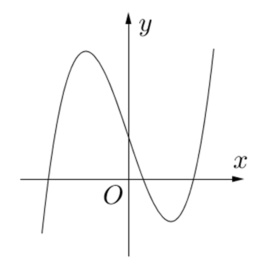
\includegraphics[scale=0.6]{toan01}\hspace*{1cm}},{\label{fig:b01}}]
bốn hàm số được liệt kê ở bốn phương án $A, B, C, D$ dưới
đây.  Hỏi hàm số đó là hàm số nào ?
\end{window}
}{
\datcot[4]
\bonpa
{\sai{$y=-x^2+x-1$.}}
{\sai{$y=-x^3+3x+1$.}}
{\dung{$y=x^3-3x+1$.}}
{\sai {$y=x^4-x^2+1$.}}
\loigiai{ 
Dựa vào đồ thị hàm số ta loại đi 2 đáp án A và C.\\
Dựa vào đồ thị hàm số ta suy ra bảng biến thiên của hàm số có dạng\\
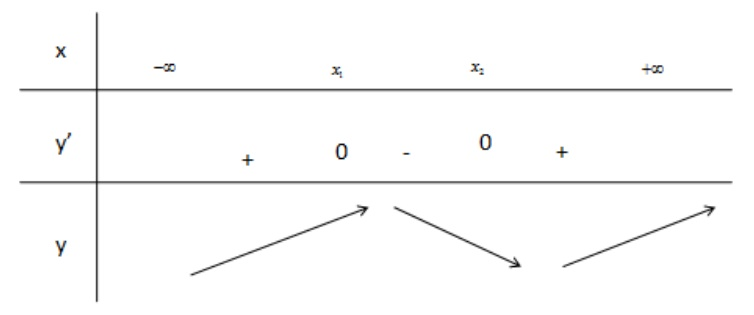
\includegraphics[scale=0.5]{gtoan01}\\
Như vậy ta thấy $y’ = 0$ có 2 nghiệm phân
 biệt và $y’$ trái dấu với hệ số của a nên hệ số $a > 0$
}
}

\baitracnghiem{abc:b02}{%
Cho hàm số $y=f(x)$ có  $\lim\limits_{x\rightarrow +\infty}f(x)=1$ và   $\lim\limits_{x\rightarrow -\infty}f(x)=-1$. Khẳng định nào sau
đây là khẳng định đúng ?
}{
\datcot[4]
\bonpa
{\sai{Đồ thị hàm số đã cho không có tiệm cận ngang.}}
{\sai{Đồ thị hàm số đã cho có đúng một tiệm cận ngang.}}
{\dung{Đồ thị hàm số đã cho có hai tiệm cận ngang là các đường thẳng  $y=1$ và  $y=-1$.}}
{\sai{Đồ thị hàm số đã cho có hai tiệm cận ngang là các đường thẳng $x=1$ và  $x=-1$.}}
\loigiai{
Vì  $\lim\limits_{x\rightarrow\infty} f(x)=1$ nên hàm số có tiệm cận ngang $y = 1$\\
Vì  $\lim\limits_{x\rightarrow-\infty} f(x)=1$ nên hàm số có tiệm cận ngang $y =-1$\\
Vậy hàm số có 2 tiệm cận ngang.
}
}

\baitracnghiem{t2017:b06}{%
Tìm giá trị nhỏ nhất của hàm số $y=\dfrac{x^2+3}{x-1}$ trên đoạn $[2;4]$.
}{
\datcot
\bonpa
{\dung{$\min_{[2;4]} y=6$.}}
{\sai{$\min_{[2;4]} y=-2$.}}
{\sai{$\min_{[2;4]} y=-3$.}}
{\sai {$\min_{[2;4]} y=\dfrac{19}{3}$.}}
\loigiai{
\begin{align*}
y&=\dfrac{x^2+3}{x-1}.\\
y'&=\dfrac{2x(x-1)-x^2-3}{(x-1)^2}=\dfrac{x^2-2x-3}{(x-1)^2}.\\
y'&=0\Leftrightarrow\left[\begin{matrix}
x=-1\quad \mbox{ loại }\\ 
x=3\quad \mbox{ thỏa mãn }\\ 
\end{matrix}\right..
\end{align*}
Có $y(2)=7; y(3)=6; y(4)=\dfrac{19}{3} \Rightarrow \min\limits_{[2;4]} y=6$.
}
}



\end{verbbox} 
\dkhung
\indebai
 \baitracnghiem{abc:b01}{%
Đường cong trong hình bên là đồ thị của một hàm số trong 
\begin{window}[0,r,{\hspace*{1cm}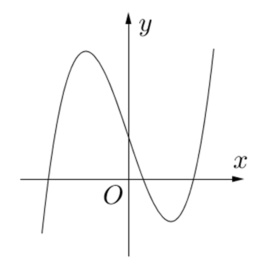
\includegraphics[scale=0.6]{toan01}\hspace*{1cm}},{\label{fig:b01}}]
bốn hàm số được liệt kê ở bốn phương án $A, B, C, D$ dưới
đây.  Hỏi hàm số đó là hàm số nào ?
\end{window}
}{
\datcot[4]
\bonpa
{\sai{$y=-x^2+x-1$.}}
{\sai{$y=-x^3+3x+1$.}}
{\dung{$y=x^3-3x+1$.}}
{\sai {$y=x^4-x^2+1$.}}
\loigiai{ 
Dựa vào đồ thị hàm số ta loại đi 2 đáp án A và C.\\
Dựa vào đồ thị hàm số ta suy ra bảng biến thiên của hàm số có dạng\\
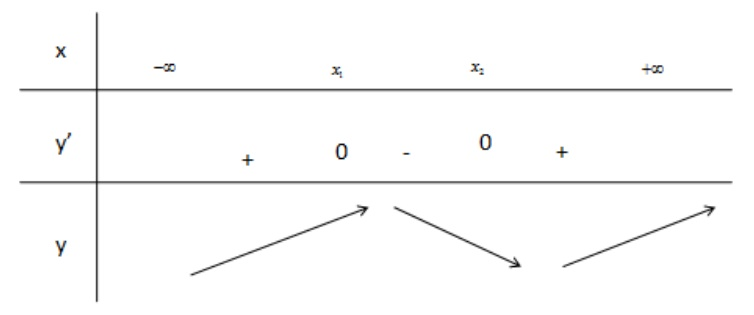
\includegraphics[scale=0.5]{gtoan01}\\
Như vậy ta thấy $y’ = 0$ có 2 nghiệm phân
 biệt và $y’$ trái dấu với hệ số của a nên hệ số $a > 0$
}
}

\baitracnghiem{abc:b02}{%
Cho hàm số $y=f(x)$ có  $\lim\limits_{x\rightarrow +\infty}f(x)=1$ và   $\lim\limits_{x\rightarrow -\infty}f(x)=-1$. Khẳng định nào sau
đây là khẳng định đúng ?
}{
\datcot[4]
\bonpa
{\sai{Đồ thị hàm số đã cho không có tiệm cận ngang.}}
{\sai{Đồ thị hàm số đã cho có đúng một tiệm cận ngang.}}
{\dung{Đồ thị hàm số đã cho có hai tiệm cận ngang là các đường thẳng  $y=1$ và  $y=-1$.}}
{\sai{Đồ thị hàm số đã cho có hai tiệm cận ngang là các đường thẳng $x=1$ và  $x=-1$.}}
\loigiai{
Vì  $\lim\limits_{x\rightarrow\infty} f(x)=1$ nên hàm số có tiệm cận ngang $y = 1$\\
Vì  $\lim\limits_{x\rightarrow-\infty} f(x)=1$ nên hàm số có tiệm cận ngang $y =-1$\\
Vậy hàm số có 2 tiệm cận ngang.
}
}

\baitracnghiem{t2017:b06}{%
Tìm giá trị nhỏ nhất của hàm số $y=\dfrac{x^2+3}{x-1}$ trên đoạn $[2;4]$.
}{
\datcot
\bonpa
{\dung{$\min_{[2;4]} y=6$.}}
{\sai{$\min_{[2;4]} y=-2$.}}
{\sai{$\min_{[2;4]} y=-3$.}}
{\sai {$\min_{[2;4]} y=\dfrac{19}{3}$.}}
\loigiai{
\begin{align*}
y&=\dfrac{x^2+3}{x-1}.\\
y'&=\dfrac{2x(x-1)-x^2-3}{(x-1)^2}=\dfrac{x^2-2x-3}{(x-1)^2}.\\
y'&=0\Leftrightarrow\left[\begin{matrix}
x=-1\quad \mbox{ loại }\\ 
x=3\quad \mbox{ thỏa mãn }\\ 
\end{matrix}\right..
\end{align*}
Có $y(2)=7; y(3)=6; y(4)=\dfrac{19}{3} \Rightarrow \min\limits_{[2;4]} y=6$.
}
}



\subsection{Xem đề bài và đáp án}
\begin{verbbox} 
 \indebaidapan
 \baitracnghiem{abc:b01}{%
Đường cong trong hình bên là đồ thị của một hàm số trong 
\begin{window}[0,r,{\hspace*{1cm}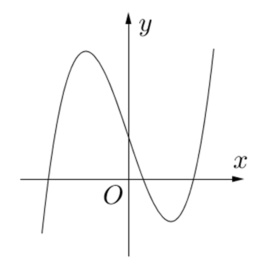
\includegraphics[scale=0.6]{toan01}\hspace*{1cm}},{\label{fig:b01}}]
bốn hàm số được liệt kê ở bốn phương án $A, B, C, D$ dưới
đây.  Hỏi hàm số đó là hàm số nào ?
\end{window}
}{
\datcot[4]
\bonpa
{\sai{$y=-x^2+x-1$.}}
{\sai{$y=-x^3+3x+1$.}}
{\dung{$y=x^3-3x+1$.}}
{\sai {$y=x^4-x^2+1$.}}
\loigiai{ 
Dựa vào đồ thị hàm số ta loại đi 2 đáp án A và C.\\
Dựa vào đồ thị hàm số ta suy ra bảng biến thiên của hàm số có dạng\\
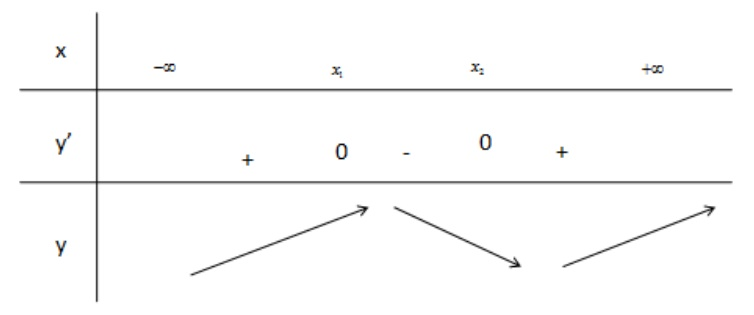
\includegraphics[scale=0.5]{gtoan01}\\
Như vậy ta thấy $y’ = 0$ có 2 nghiệm phân
 biệt và $y’$ trái dấu với hệ số của a nên hệ số $a > 0$
}
}

\baitracnghiem{abc:b02}{%
Cho hàm số $y=f(x)$ có  $\lim\limits_{x\rightarrow +\infty}f(x)=1$ và   $\lim\limits_{x\rightarrow -\infty}f(x)=-1$. Khẳng định nào sau
đây là khẳng định đúng ?
}{
\datcot[4]
\bonpa
{\sai{Đồ thị hàm số đã cho không có tiệm cận ngang.}}
{\sai{Đồ thị hàm số đã cho có đúng một tiệm cận ngang.}}
{\dung{Đồ thị hàm số đã cho có hai tiệm cận ngang là các đường thẳng  $y=1$ và  $y=-1$.}}
{\sai{Đồ thị hàm số đã cho có hai tiệm cận ngang là các đường thẳng $x=1$ và  $x=-1$.}}
\loigiai{
Vì  $\lim\limits_{x\rightarrow\infty} f(x)=1$ nên hàm số có tiệm cận ngang $y = 1$\\
Vì  $\lim\limits_{x\rightarrow-\infty} f(x)=1$ nên hàm số có tiệm cận ngang $y =-1$\\
Vậy hàm số có 2 tiệm cận ngang.
}
}

\baitracnghiem{t2017:b06}{%
Tìm giá trị nhỏ nhất của hàm số $y=\dfrac{x^2+3}{x-1}$ trên đoạn $[2;4]$.
}{
\datcot
\bonpa
{\dung{$\min_{[2;4]} y=6$.}}
{\sai{$\min_{[2;4]} y=-2$.}}
{\sai{$\min_{[2;4]} y=-3$.}}
{\sai {$\min_{[2;4]} y=\dfrac{19}{3}$.}}
\loigiai{
\begin{align*}
y&=\dfrac{x^2+3}{x-1}.\\
y'&=\dfrac{2x(x-1)-x^2-3}{(x-1)^2}=\dfrac{x^2-2x-3}{(x-1)^2}.\\
y'&=0\Leftrightarrow\left[\begin{matrix}
x=-1\quad \mbox{ loại }\\ 
x=3\quad \mbox{ thỏa mãn }\\ 
\end{matrix}\right..
\end{align*}
Có $y(2)=7; y(3)=6; y(4)=\dfrac{19}{3} \Rightarrow \min\limits_{[2;4]} y=6$.
}
}



\end{verbbox} 
\dkhung
\indebaidapan
 \baitracnghiem{abc:b01}{%
Đường cong trong hình bên là đồ thị của một hàm số trong 
\begin{window}[0,r,{\hspace*{1cm}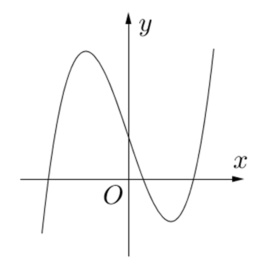
\includegraphics[scale=0.6]{toan01}\hspace*{1cm}},{\label{fig:b01}}]
bốn hàm số được liệt kê ở bốn phương án $A, B, C, D$ dưới
đây.  Hỏi hàm số đó là hàm số nào ?
\end{window}
}{
\datcot[4]
\bonpa
{\sai{$y=-x^2+x-1$.}}
{\sai{$y=-x^3+3x+1$.}}
{\dung{$y=x^3-3x+1$.}}
{\sai {$y=x^4-x^2+1$.}}
\loigiai{ 
Dựa vào đồ thị hàm số ta loại đi 2 đáp án A và C.\\
Dựa vào đồ thị hàm số ta suy ra bảng biến thiên của hàm số có dạng\\
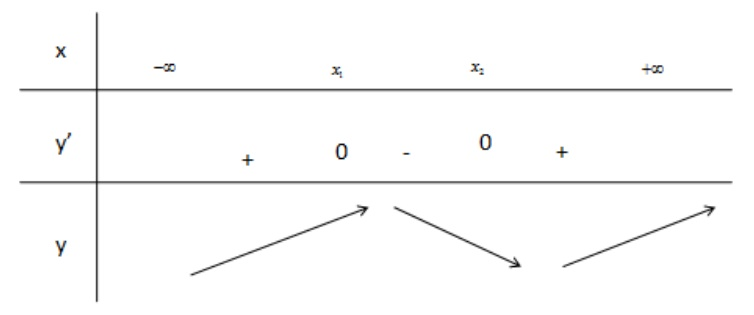
\includegraphics[scale=0.5]{gtoan01}\\
Như vậy ta thấy $y’ = 0$ có 2 nghiệm phân
 biệt và $y’$ trái dấu với hệ số của a nên hệ số $a > 0$
}
}

\baitracnghiem{abc:b02}{%
Cho hàm số $y=f(x)$ có  $\lim\limits_{x\rightarrow +\infty}f(x)=1$ và   $\lim\limits_{x\rightarrow -\infty}f(x)=-1$. Khẳng định nào sau
đây là khẳng định đúng ?
}{
\datcot[4]
\bonpa
{\sai{Đồ thị hàm số đã cho không có tiệm cận ngang.}}
{\sai{Đồ thị hàm số đã cho có đúng một tiệm cận ngang.}}
{\dung{Đồ thị hàm số đã cho có hai tiệm cận ngang là các đường thẳng  $y=1$ và  $y=-1$.}}
{\sai{Đồ thị hàm số đã cho có hai tiệm cận ngang là các đường thẳng $x=1$ và  $x=-1$.}}
\loigiai{
Vì  $\lim\limits_{x\rightarrow\infty} f(x)=1$ nên hàm số có tiệm cận ngang $y = 1$\\
Vì  $\lim\limits_{x\rightarrow-\infty} f(x)=1$ nên hàm số có tiệm cận ngang $y =-1$\\
Vậy hàm số có 2 tiệm cận ngang.
}
}

\baitracnghiem{t2017:b06}{%
Tìm giá trị nhỏ nhất của hàm số $y=\dfrac{x^2+3}{x-1}$ trên đoạn $[2;4]$.
}{
\datcot
\bonpa
{\dung{$\min_{[2;4]} y=6$.}}
{\sai{$\min_{[2;4]} y=-2$.}}
{\sai{$\min_{[2;4]} y=-3$.}}
{\sai {$\min_{[2;4]} y=\dfrac{19}{3}$.}}
\loigiai{
\begin{align*}
y&=\dfrac{x^2+3}{x-1}.\\
y'&=\dfrac{2x(x-1)-x^2-3}{(x-1)^2}=\dfrac{x^2-2x-3}{(x-1)^2}.\\
y'&=0\Leftrightarrow\left[\begin{matrix}
x=-1\quad \mbox{ loại }\\ 
x=3\quad \mbox{ thỏa mãn }\\ 
\end{matrix}\right..
\end{align*}
Có $y(2)=7; y(3)=6; y(4)=\dfrac{19}{3} \Rightarrow \min\limits_{[2;4]} y=6$.
}
}



\setcounter{question}{0}
\subsection{Đề bài, đánh dấu đáp án và lời giải }
\begin{verbbox} 
 \indebailoigiai
 \baitracnghiem{abc:b01}{%
Đường cong trong hình bên là đồ thị của một hàm số trong 
\begin{window}[0,r,{\hspace*{1cm}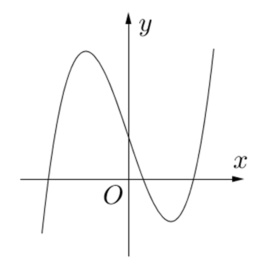
\includegraphics[scale=0.6]{toan01}\hspace*{1cm}},{\label{fig:b01}}]
bốn hàm số được liệt kê ở bốn phương án $A, B, C, D$ dưới
đây.  Hỏi hàm số đó là hàm số nào ?
\end{window}
}{
\datcot[4]
\bonpa
{\sai{$y=-x^2+x-1$.}}
{\sai{$y=-x^3+3x+1$.}}
{\dung{$y=x^3-3x+1$.}}
{\sai {$y=x^4-x^2+1$.}}
\loigiai{ 
Dựa vào đồ thị hàm số ta loại đi 2 đáp án A và C.\\
Dựa vào đồ thị hàm số ta suy ra bảng biến thiên của hàm số có dạng\\
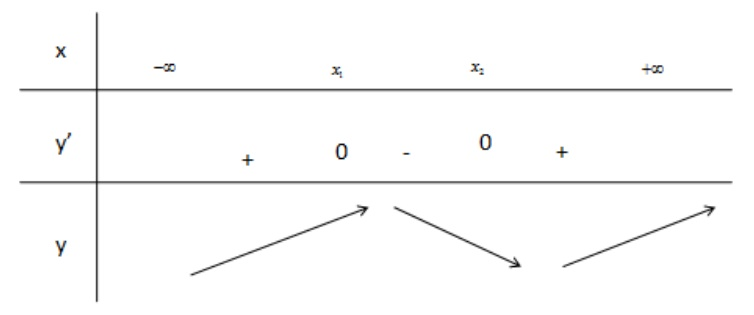
\includegraphics[scale=0.5]{gtoan01}\\
Như vậy ta thấy $y’ = 0$ có 2 nghiệm phân
 biệt và $y’$ trái dấu với hệ số của a nên hệ số $a > 0$
}
}

\baitracnghiem{abc:b02}{%
Cho hàm số $y=f(x)$ có  $\lim\limits_{x\rightarrow +\infty}f(x)=1$ và   $\lim\limits_{x\rightarrow -\infty}f(x)=-1$. Khẳng định nào sau
đây là khẳng định đúng ?
}{
\datcot[4]
\bonpa
{\sai{Đồ thị hàm số đã cho không có tiệm cận ngang.}}
{\sai{Đồ thị hàm số đã cho có đúng một tiệm cận ngang.}}
{\dung{Đồ thị hàm số đã cho có hai tiệm cận ngang là các đường thẳng  $y=1$ và  $y=-1$.}}
{\sai{Đồ thị hàm số đã cho có hai tiệm cận ngang là các đường thẳng $x=1$ và  $x=-1$.}}
\loigiai{
Vì  $\lim\limits_{x\rightarrow\infty} f(x)=1$ nên hàm số có tiệm cận ngang $y = 1$\\
Vì  $\lim\limits_{x\rightarrow-\infty} f(x)=1$ nên hàm số có tiệm cận ngang $y =-1$\\
Vậy hàm số có 2 tiệm cận ngang.
}
}

\baitracnghiem{t2017:b06}{%
Tìm giá trị nhỏ nhất của hàm số $y=\dfrac{x^2+3}{x-1}$ trên đoạn $[2;4]$.
}{
\datcot
\bonpa
{\dung{$\min_{[2;4]} y=6$.}}
{\sai{$\min_{[2;4]} y=-2$.}}
{\sai{$\min_{[2;4]} y=-3$.}}
{\sai {$\min_{[2;4]} y=\dfrac{19}{3}$.}}
\loigiai{
\begin{align*}
y&=\dfrac{x^2+3}{x-1}.\\
y'&=\dfrac{2x(x-1)-x^2-3}{(x-1)^2}=\dfrac{x^2-2x-3}{(x-1)^2}.\\
y'&=0\Leftrightarrow\left[\begin{matrix}
x=-1\quad \mbox{ loại }\\ 
x=3\quad \mbox{ thỏa mãn }\\ 
\end{matrix}\right..
\end{align*}
Có $y(2)=7; y(3)=6; y(4)=\dfrac{19}{3} \Rightarrow \min\limits_{[2;4]} y=6$.
}
}



\end{verbbox} 
\dkhung
\indebailoigiai
 \baitracnghiem{abc:b01}{%
Đường cong trong hình bên là đồ thị của một hàm số trong 
\begin{window}[0,r,{\hspace*{1cm}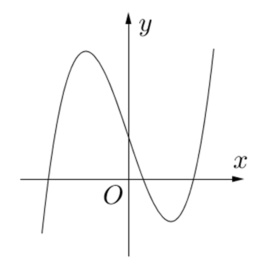
\includegraphics[scale=0.6]{toan01}\hspace*{1cm}},{\label{fig:b01}}]
bốn hàm số được liệt kê ở bốn phương án $A, B, C, D$ dưới
đây.  Hỏi hàm số đó là hàm số nào ?
\end{window}
}{
\datcot[4]
\bonpa
{\sai{$y=-x^2+x-1$.}}
{\sai{$y=-x^3+3x+1$.}}
{\dung{$y=x^3-3x+1$.}}
{\sai {$y=x^4-x^2+1$.}}
\loigiai{ 
Dựa vào đồ thị hàm số ta loại đi 2 đáp án A và C.\\
Dựa vào đồ thị hàm số ta suy ra bảng biến thiên của hàm số có dạng\\
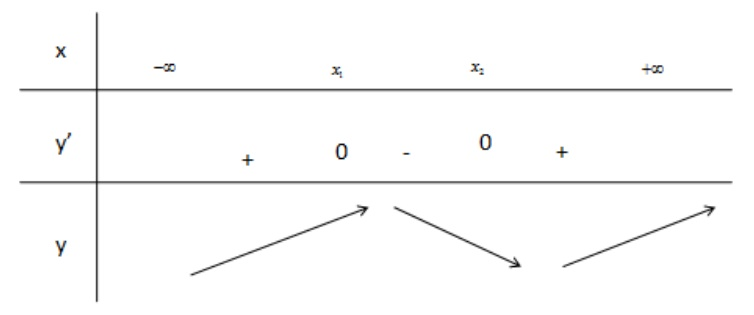
\includegraphics[scale=0.5]{gtoan01}\\
Như vậy ta thấy $y’ = 0$ có 2 nghiệm phân
 biệt và $y’$ trái dấu với hệ số của a nên hệ số $a > 0$
}
}

\baitracnghiem{abc:b02}{%
Cho hàm số $y=f(x)$ có  $\lim\limits_{x\rightarrow +\infty}f(x)=1$ và   $\lim\limits_{x\rightarrow -\infty}f(x)=-1$. Khẳng định nào sau
đây là khẳng định đúng ?
}{
\datcot[4]
\bonpa
{\sai{Đồ thị hàm số đã cho không có tiệm cận ngang.}}
{\sai{Đồ thị hàm số đã cho có đúng một tiệm cận ngang.}}
{\dung{Đồ thị hàm số đã cho có hai tiệm cận ngang là các đường thẳng  $y=1$ và  $y=-1$.}}
{\sai{Đồ thị hàm số đã cho có hai tiệm cận ngang là các đường thẳng $x=1$ và  $x=-1$.}}
\loigiai{
Vì  $\lim\limits_{x\rightarrow\infty} f(x)=1$ nên hàm số có tiệm cận ngang $y = 1$\\
Vì  $\lim\limits_{x\rightarrow-\infty} f(x)=1$ nên hàm số có tiệm cận ngang $y =-1$\\
Vậy hàm số có 2 tiệm cận ngang.
}
}

\baitracnghiem{t2017:b06}{%
Tìm giá trị nhỏ nhất của hàm số $y=\dfrac{x^2+3}{x-1}$ trên đoạn $[2;4]$.
}{
\datcot
\bonpa
{\dung{$\min_{[2;4]} y=6$.}}
{\sai{$\min_{[2;4]} y=-2$.}}
{\sai{$\min_{[2;4]} y=-3$.}}
{\sai {$\min_{[2;4]} y=\dfrac{19}{3}$.}}
\loigiai{
\begin{align*}
y&=\dfrac{x^2+3}{x-1}.\\
y'&=\dfrac{2x(x-1)-x^2-3}{(x-1)^2}=\dfrac{x^2-2x-3}{(x-1)^2}.\\
y'&=0\Leftrightarrow\left[\begin{matrix}
x=-1\quad \mbox{ loại }\\ 
x=3\quad \mbox{ thỏa mãn }\\ 
\end{matrix}\right..
\end{align*}
Có $y(2)=7; y(3)=6; y(4)=\dfrac{19}{3} \Rightarrow \min\limits_{[2;4]} y=6$.
}
}



%  \baitracnghiem{de20170120:b01}{
Đường thẳng nào dưới đây là tiệm cận đứng của đồ thị hàm số $y=\dfrac{2x+1}{x+1}$
}{\datcot\bonpa
{\sai{$x=1$.}}
{\sai{$y=-1$.}}
{\sai{$y=2$.}}
{\dung {$x=-1$.}}
\loigiai{Tập xác định $D=\mathbb{R}\setminus\left\{ -1 \right\}$ và $\displaystyle\lim_{x\to -1^+}\dfrac{2x+1}{x+1}=-\infty ;\displaystyle\lim_{x\to -1^+}\dfrac{2x+1}{x+1}=+\infty$ \\ nên $x=-1$ là phương trình tiệm cận đứng.
}
}

\baitracnghiem{de20170120:b02}{
Đồ thị của hàm số $y=x^4-2x^2+2$ và đồ thị của hàm số $y=-x^2+4$ có tất cả bao nhiêu điểm chung ?
}{\datcot\bonpa
{\sai{$0$.}}
{\sai{$4$.}}
{\sai{$1$.}}
{\dung {$2$.}}
\loigiai{${{x}^{4}}-2{{x}^{2}}+2=-{{x}^{2}}+4\Leftrightarrow {{x}^{4}}-{{x}^{2}}-2=0\Leftrightarrow \left[ \begin{aligned}  & x=\sqrt{2} \\  & x=-\sqrt{2}  \end{aligned} \right.$
}
}

\baitracnghiem{de20170120:b03}{
Cho hàm số $y=f(x)$ xác định, liên tục trên đoạn $[-2;2]$ 
\begin{window}[0,r,{\hspace*{1cm}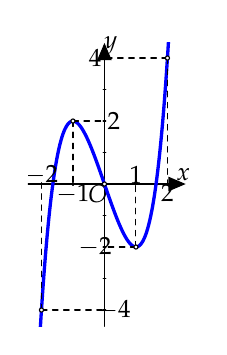
\begin{tikzpicture}[line cap=round,line join=round,>=triangle 45,x=0.8cm,y=0.8cm,scale=.5]
\begin{small}
\draw[->,color=black] (-2.42,0.) -- (2.58,0.);
\foreach \x in {-2.,-1.,1.,2.}
\draw[shift={(\x,0)},color=black] (0pt,-1pt) -- (0pt,1pt);
\draw[color=black] (2.5,0.3) node { $x$};
\draw[->,color=black] (0.,-4.52) -- (0.,4.48);
\foreach \y in {-4.,-3.,-2.,-1.,1.,2.,3.,4.}
\draw[shift={(0,\y)},color=black] (1pt,0pt) -- (-1pt,0pt);
\draw[color=black] (0.2,4.4) node{ $y$};
\draw[color=black] (-0.2,-0.3) node{ $O$};
\clip(-2.42,-4.52) rectangle (2.58,4.48);
\draw[line width=1.2pt,color=blue,smooth,samples=100,domain=-2.42:2.58] plot(\x,{((\x)^(5.0)+7.0*(\x)^(3.0)-26.0*(\x))/9.0});
\draw [dash pattern=on 2pt off 2pt] (-1.,2.)-- (0.,2.);
\draw [dash pattern=on 2pt off 2pt] (-1.,2.)-- (-1.,0.);
\draw [dash pattern=on 2pt off 2pt] (1.,-2.)-- (1.,0.);
\draw [dash pattern=on 2pt off 2pt] (1.,-2.)-- (0.,-2.);
\draw [dash pattern=on 2pt off 2pt] (-2.,-4.)-- (0.,-4.);
\draw [dash pattern=on 2pt off 2pt] (-2.,-4.)-- (-2.,0.);
\draw [dash pattern=on 2pt off 2pt] (2.,4.)-- (0.,4.);
\draw [dash pattern=on 2pt off 2pt] (2.,4.)-- (2.,0.);
\draw [fill=white,draw=black] (-1.,2.) circle (1.50pt);
\draw [fill=white,draw=black] (0.,0.) circle (1.50pt);
\draw [fill=white,draw=black] (1.,-2.) circle (1.50pt);
\draw [fill=white,draw=black] (2.,4.) circle (1.50pt);
\draw [fill=white,draw=black] (-2.,-4.) circle (1.50pt);
\draw[color=black] (-0.3,4.) node{ $4$};
\draw[color=black] (0.3,2.) node{ $2$};
\draw[color=black] (0.3,-4.) node{ $-4$};
\draw[color=black] (-0.3,-2.) node{ $-2$};
\draw[color=black] (2.,-.3) node{ $2$};
\draw[color=black] (-2.,.3) node{ $-2$};
\draw[color=black] (1.,.3) node{ $1$};
\draw[color=black] (-1.,-.3) node{ $-1$};
\end{small}
\end{tikzpicture}\hspace*{1cm}},{\label{fig:anh03}}]
và có đồ thị là đường cong trong hình vẽ bên. Hàm số $f(x)$ đạt cực đại tại điểm nào dưới đây ?
\end{window}\examvspace*{0.5cm}
}{\datcot[4]\bonpa
{\sai{$x=2$.}}
{\dung{$x=-1$.}}
{\sai{$x=1$.}}
{\sai {$x=2$.}}
\loigiai{Đồ thị có điểm cực đại $(-1;2)$ nên hàm số $f(x)$ đạt cực đại tại $x=-1$
}
}

\baitracnghiem{de20170120:b04}{
Cho hàm số $y=x^3-2x^2+x+1$. Mệnh đề nào dưới đây đúng ?
}{\datcot[2]\bonpa
{\dung{Hàm số nghịch biến trên khoảng $\left(\frac13; 1\right)$.}}
{\sai{Hàm số nghịch biến trên khoảng $\left(-\infty; \frac13\right)$.}}
{\sai{Hàm số đồng biến trên khoảng $\left(\frac13;1\right)$.}}
{\sai {Hàm số nghịch biến trên khoảng $\left(1;+\infty\right)$.}}
\loigiai{Ta có $y'=3x^2-4x+1\Rightarrow y'=0\Leftrightarrow x=1$ hoặc $x=\dfrac{1}{3}$. Nên $y'<0 ~\forall x\in\left(\frac13; 1\right)$
}
}

\baitracnghiem{de20170120:b05}{
Cho hàm số $y=f(x)$ xác định trên $\mathbb R\setminus \{0\}$,
\begin{window}[0,r,{\hspace*{1cm}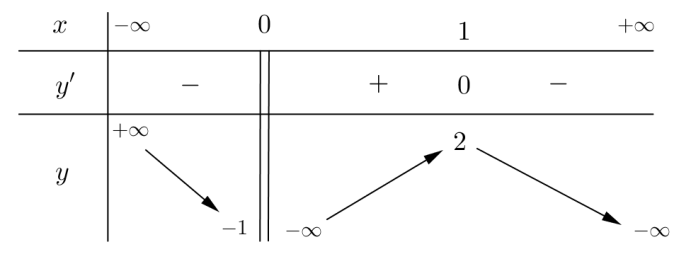
\includegraphics[scale=0.45]{anh05}\hspace*{0.\linewidth}},{\label{fig:anh05}}]
liên tục trên mỗi khoảng xác định và có bảng biến thiên như sau. Tìm tập hợp tất cả các giá trị của tham số thực m sao cho phương trình  $ f (x)= m $ có ba nghiệm thực phân biệt.
\end{window}\examvspace*{0.8cm}
}{\datcot\bonpa
{\sai{$[-1;2]$.}}
{\dung{$(-1;2)$.}}
{\sai{$(-1;2]$.}}
{\sai{$(-\infty;2]$.}}
\loigiai{Nhìn bảng biến thiên ta thấy $f\left( x \right)=m$ có ba nghiệm phân biệt khi và chỉ khi $-1<m<2$
}
}

\baitracnghiem{de20170120:b06}{
Cho hàm số $y=\dfrac{x^2+3}{x+1} $. Mệnh đề nào dưới đây đúng ?
}{\datcot[2]\bonpa
{\sai{Cực tiểu của hàm số bằng $-3$.}}
{\sai{Cực tiểu của hàm số bằng $1$.}}
{\sai{Cực tiểu của hàm số bằng $-6$.}}
{\dung{Cực tiểu của hàm số bằng $2$.}}
\loigiai{Ta có: $y'=\dfrac{x^2+2x-3}{\left( x+1 \right)^2}$; $y'=0\Leftrightarrow x^2+2x-3=0\Leftrightarrow \left[ \begin{aligned} & x=-3 \\ & x=1 \end{aligned} \right.$\\
Lập bảng biến thiên. 
Thấy hàm số đạt cực tiểu tại $x=1$ và giá trị cực tiểu bằng $y(1)=2$
}
}

\baitracnghiem{de20170120:b07}{
Một vật chuyển động theo quy luật $s=-\dfrac12t^3+9t^2$, với $t$ (giây) là khoảng thời gian tính từ lúc vật bắt đầu chuyển động và $s$ (mét) là quãng đường vật đi được trong khoảng thời gian đó. Hỏi trong khoảng thời gian 10 giây, kể từ lúc bắt đầu chuyển động, vận tốc lớn nhất của vật đạt được bằng bao nhiêu ?
}{\datcot\bonpa
{\sai{$216 (m/s)$.}}
{\sai{$30 (m/s)$.}}
{\sai{$400 (m/s)$.}}
{\dung{$54 (m/s)$.}}
\loigiai{Vận tốc tại thời điểm $t$ là $v(t)=s'(t)=-\dfrac{3}{2}t^2+18t$\\ 
nên vận tốc lớn nhất của vật đạt được khi $v'(t)=-3t+18=0\Leftrightarrow t=6$.
}
}

\baitracnghiem{de20170120:b08}{
Tìm tất cả các tiệm cận đứng của đồ thị hàm số $y=\dfrac{2x-1-\sqrt{x^2+x+3}}{x^2-5x+6}$
}{\datcot\bonpa
{\sai{$x=-3$ và $x=-2$.}}
{\sai{$x=-3$.}}
{\sai{$x=3$ và $x=2$.}}
{\dung{$x=3$.}}
\loigiai{Tập xác định $D=\mathbb{R}\setminus\left\{ 2;3 \right\}$\\ 
nhưng $\displaystyle\lim_{x\to 2^+}\dfrac{2x-1-\sqrt{{{x}^{2}}+x+3}}{{{x}^{2}}-5x+6}=-\dfrac{7}{6} ; \displaystyle\lim_{x\to 2^-}\dfrac{2x-1-\sqrt{{{x}^{2}}+x+3}}{{{x}^{2}}-5x+6}=-\dfrac{7}{6}$ \\
và $\displaystyle\lim_{x\to 3^+}\dfrac{2x-1-\sqrt{{{x}^{2}}+x+3}}{{{x}^{2}}-5x+6}=+\infty ;\displaystyle\lim_{x\to 3^-}\dfrac{2x-1-\sqrt{{{x}^{2}}+x+3}}{{{x}^{2}}-5x+6}=-\infty $\\ nên chỉ $x=3$ là phương trình tiệm cận đứng (Chú ý: Dùng Casio để tìm $\lim$)
}
}

\baitracnghiem{de20170120:b09}{
Tìm tập hợp tất cả các giá trị của tham số thực $m$ để hàm số $y=\ln\left(x^2+1\right)-mx+1$ đồng biến trên khoảng $(-\infty;+\infty)$
}{\datcot\bonpa
{\dung{$(-\infty;-1]$.}}
{\sai{$(-\infty;-1)$.}}
{\sai{$[-1;1]$.}}
{\sai{$[1;+\infty)$.}}
\loigiai{$y=\ln \left( x^2+1 \right)-mx+1$ đồng biến trên $\left( -\infty ;+\infty  \right) \Leftrightarrow  y'=\dfrac{2x}{x^2+1}-m \ge 0,\forall x\in \left( -\infty ;+\infty  \right)$.\\
$\Leftrightarrow g(x)=\dfrac{2x}{x^2+1}\ge m,\forall x\in \left( -\infty ;+\infty  \right)$. Mà $g'(x)=\dfrac{-2x^2+2}{\left( x^2+1 \right)^2}=0\Leftrightarrow x=\pm 1$\\
Dựa vào bảng biến thiên của $g(x)$ ta có: $\dfrac{2x}{x^2+1}\ge m,\forall x\in \left( -\infty ;+\infty  \right)\Leftrightarrow m\le -1$ 
}
}

\baitracnghiem{de20170120:b10}{
Biết $M(0;2), N(2;-2)$ là các điểm cực trị của đồ thị hàm số $y=ax^3+bx^2+cx+d$. Tính giá trị của hàm số tại $x=-2$.
}{\datcot\bonpa
{\sai{$y(-2)=2$.}}
{\sai{$y(-2)=22$.}}
{\sai{$y(-2)=6$.}}
{\dung{$y(-2)=-18$.}}
\loigiai{Ta có: ${y}'=3a{{x}^{2}}+2bx+c$.
Vì $M(0;2)$,$N(2;-2)$ là các điểm cực trị của đồ thị hàm số nên: \\
$\left\{ \begin{aligned}
  & {y}'(0)=0 \\ 
 & {y}'(2)=0 \\ 
\end{aligned} \right.\Leftrightarrow \left\{ \begin{aligned}
  & c=0 \\ 
 & 12a+4b+c=0 \\ 
\end{aligned} \right.\quad(1)$;\qquad$\left\{ \begin{aligned}
  & y(0)=2 \\ 
 & y(2)=-2 \\ 
\end{aligned} \right.\Leftrightarrow \left\{ \begin{aligned}
  & d=2 \\ 
 & 8a+4b+2c+d=-2 \\ 
\end{aligned} \right.\quad(2)$\\
Từ $(1)$ và $(2)$ suy ra:$a=1;b=-3;c=0;d=2\Rightarrow y={{x}^{3}}-3{{x}^{2}}+2\Rightarrow y(-2)=-18$.
}
}

\baitracnghiem{de20170120:b11}{
Cho hàm số $y=ax^3+bx^2+cx+d$ có
\begin{window}[0,r,{\hspace*{1cm}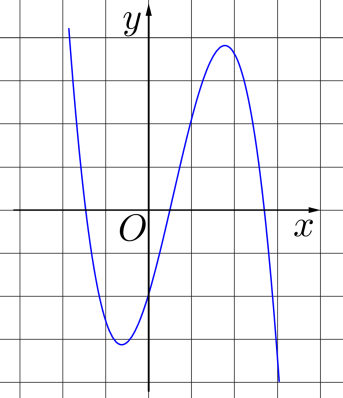
\includegraphics[scale=0.3]{anh11}\hspace*{1cm}},{\label{fig:anh11}}]
đồ thị như hình vẽ bên. Mệnh đề nào dưới đây
đúng ?
\end{window}\examvspace*{0.5cm}
}{\datcot[4]\bonpa
{\dung{$a<0,b>0,c>0,d<0$.}}
{\sai{$a<0,b<0,c>0,d<0$.}}
{\sai{$a<0,b<0,c<0,d>0$.}}
{\sai{$a<0,b>0,c<0,d<0$.}}
\loigiai{Dựa vào 2 nhánh vô tận của đồ thị suy ra hệ số $a<0$.\\ 
Dựa vào giao điểm đồ thị với trục tụng ở dưới nên $d<0$\\ 
Dựa vào hoành độ 2 điểm cực trị trái dấu nên $3a.c<0\Rightarrow c>0$\\ 
Trung điểm của 2  điểm cực trị có hoành độ dương nên
$\dfrac{-b}{3a}>0\Rightarrow b>0$.
}
}
\baitracnghiem{de20170120:b12}{
Với các số thực dương $a, b$ bất kì. Mệnh đề nào dưới đây đúng ?
}{\datcot\bonpa
{\dung{$\ln(ab)=\ln a+\ln b$.}}
{\sai{$\ln(ab)=\ln a.\ln b$.}}
{\sai{$\ln\dfrac ab=\dfrac{\ln a}{\ln b}$.}}
{\sai{$\ln\dfrac ab=\ln b-\ln a$.}}
\loigiai{log tích bằng tổng log, log thương bằng hiệu log tử log mẫu.
}
}
\baitracnghiem{de20170120:b13}{
Tìm nghiệm của phương trình $3^{x-1}=27.$
}{\datcot\bonpa
{\sai{$x=9$.}}
{\sai{$x=3$.}}
{\dung{$x=4$.}}
{\sai{$x=10$.}}
\loigiai{$3^{x-1}=27\Leftrightarrow 3^{x-1}=3^3\Leftrightarrow x-1=3\Leftrightarrow x=4$
}
}
\baitracnghiem{de20170120:b14}{
Số lượng của loại vi khuẩn $A$ trong một phòng thí nghiệm được tính theo công thức $s(t)=s(0).2^t$,  trong đó $s(0)$ là số lượng vi khuẩn A lúc ban đầu, $s(t)$ là số lượng vi khuẩn $A$ có sau $t$ phút. Biết sau 3 phút thì số lượng vi khuẩn $A$ là 625 nghìn con. Hỏi sau bao lâu, kể từ lúc ban đầu, số lượng vi khuẩn $A$ là 10 triệu con ?
}{\datcot\bonpa
{\sai{48 phút.}}
{\sai{19 phút.}}
{\dung{7 phút.}}
{\sai{12 phút.}}
\loigiai{$s\left( 3 \right)=s\left( 0 \right).2^3\Rightarrow s\left( 0 \right)=\dfrac{s\left( 3 \right)}{2^3}=78125$. $s\left( t \right)=\dfrac{10000000}{78125}=128\Rightarrow t=7$
}
}
\baitracnghiem{de20170120:b15}{
Cho biểu thức $P=\sqrt[4]{x.\sqrt[3]{x^2.\sqrt{x^3}}}$, với $x>0$. Mệnh đề nào dưới đây đúng ?
}{\datcot\bonpa
{\sai{$P=x^{\frac12}$.}}
{\dung{$P=x^{\frac{13}{24}}$.}}
{\sai{$P=x^{\frac14}$.}}
{\sai{$P=x^{\frac23}$.}}
\loigiai{$P=\sqrt[4]{x.\sqrt[3]{x^2.\sqrt{x^3}}}=\sqrt[4]{x.\sqrt[3]{x^2.x^{\frac{3}{2}}}}=\sqrt[4]{x.\sqrt[3]{x^{\frac{7}{2}}}}=\sqrt[4]{x.x^{\frac{7}{6}}}=\sqrt[4]{x^{\frac{13}{6}}}=x^{\frac{13}{24}}$. 
}
}
\baitracnghiem{de20170120:b16}{
Với các số thực dương $a, b$ bất kì. Mệnh đề nào dưới đây đúng ?
}{\datcot[2]\bonpa
{\dung{$\Rightarrow \left\{ \begin{aligned}
  & x+1>0 \\ 
 & 2x-1>0 
\end{aligned} \right.\Leftrightarrow \left\{ \begin{aligned}
  & x>-1 \\ 
 & x>\frac{1}{2} 
\end{aligned} \right.\Rightarrow x>\dfrac{1}{2}$.}}
{\sai{${{\log }_{2}}\left( \frac{2{{a}^{3}}}{b} \right)=1+\frac{1}{3}{{\log }_{2}}a-{{\log }_{2}}_{\,}b$.}}
{\sai{${{\log }_{2}}\left( \frac{2{{a}^{3}}}{b} \right)=1+3{{\log }_{2}}a+{{\log }_{2}}_{\,}b$.}}
{\sai{${{\log }_{2}}\left( \frac{2{{a}^{3}}}{b} \right)=1+\frac{1}{3}{{\log }_{2}}a+{{\log }_{2}}_{\,}b$.}}
\loigiai{${{\log }_{2}}\left( \frac{2{{a}^{3}}}{b} \right)={{\log }_{2}}\left( 2{{a}^{3}} \right)-{{\log }_{2}}\left( b \right)={{\log }_{2}}2+{{\log }_{2}}{{a}^{3}}-{{\log }_{2}}b=1+3{{\log }_{2}}a-{{\log }_{\,}}b$.}
}
\baitracnghiem{de20170120:b17}{
Tìm tập nghiệm $S$ của bất phương trình ${{\log }_{\frac{1}{2}}}(x+1)<{{\log }_{\frac{1}{2}}}\left( 2x-1 \right)$ 
}{\datcot\bonpa
{\sai{$S=\left( 2;+\infty  \right)$.}}
{\sai{$S=\left( -\infty ;2 \right)$.}}
{\dung{$S=\left( \frac{1}{2};2 \right)$.}}
{\sai{$S=\left( -1;2 \right)$.}}
\loigiai{ĐKXĐ:$\left\{ \begin{aligned}
  & x+1>0 \\ 
 & 2x-1>0 \\ 
\end{aligned} \right.\Leftrightarrow \left\{ \begin{aligned}
  & x>-1 \\ 
 & x>\frac{1}{2} \\ 
\end{aligned} \right.\Rightarrow x>\frac{1}{2}\quad (*)$\\
${{\log }_{\frac{1}{2}}}(x+1)<{{\log }_{\frac{1}{2}}}\left( 2x-1 \right)\Leftrightarrow x+1>2x-1\Leftrightarrow x-2<0\Leftrightarrow x<2$
Kết hợp $(*) \Rightarrow S=\left( \frac{1}{2};2 \right)$
}
}
\baitracnghiem{de20170120:b18}{
Tính đạo hàm của hàm số $y=\ln \left( 1+\sqrt{x+1} \right)$. 
}{\datcot[2]\bonpa
{\dung{${y}'=\dfrac{1}{2\sqrt{x+1}\left( 1+\sqrt{x+1} \right)}$.}}
{\sai{${y}'=\dfrac{1}{1+\sqrt{x+1}}$.}}
{\sai{${y}'=\dfrac{1}{\sqrt{x+1}\left( 1+\sqrt{x+1} \right)}$.}}
{\sai{${y}'=\dfrac{2}{\sqrt{x+1}\left( 1+\sqrt{x+1} \right)}$.}}
\loigiai{ 
${{\left( \ln \left( 1+\sqrt{x+1} \right) \right)}^{\prime }}=\dfrac{{{\left( 1+\sqrt{x+1} \right)}^{\prime }}}{1+\sqrt{x+1}}=\dfrac{1}{2\sqrt{x+1}\left( 1+\sqrt{x+1} \right)}$ 
}
}
\baitracnghiem{de20170120:b19}{
Cho ba số thực dương $a,\,b,\,c$ khác $1$. 
\begin{window}[0,r,{\hspace*{1cm}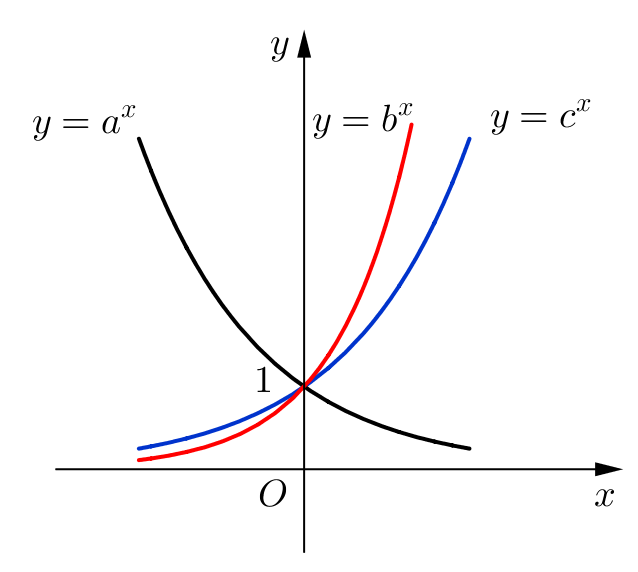
\includegraphics[scale=0.25]{anh19}\hspace*{1cm}},{\label{fig:anh19}}]
Đồ thị các hàm số $y=a^x$, $y=b^x$, $y=c^x$ được cho trong hình vẽ bên. Mệnh đề nào dưới đây  đúng?
\end{window}\examvspace*{0.cm}
}{\datcot[4]\bonpa
{\sai{$a<b<c$.}}
{\dung{$a<c<b$.}}
{\sai{$b<c<a$.}}
{\sai{$c<a<b$.}}
\loigiai{Từ đồ thị suy ra $0<a<1<c<b$
}
}
\baitracnghiem{de20170120:b20}{
Tìm tập hợp các giá trị của tham số thực $m$ để phương trình ${{6}^{x}}+\left( 3-m \right){{2}^{x}}-m=0$ có nghiệm thuộc khoảng $\left( 0;\,1 \right)$.
}{\datcot\bonpa
{\sai{$\left[ 3;\,4 \right]$.}}
{\sai{$\left[ 2;\,4 \right]$.}}
{\dung{$\left( 2;\,4 \right)$.}}
{\sai{$\left( 3;4 \right)$.}}
\loigiai{Ta có: ${{6}^{x}}+\left( 3-m \right){{2}^{x}}-m=0$ $\left( 1 \right)\Leftrightarrow \dfrac{{{6}^{x}}+{{3.2}^{x}}}{{{2}^{x}}+1}=m$ \\
Xét hàm số $f\left( x \right)=\dfrac{{{6}^{x}}+{{3.2}^{x}}}{{{2}^{x}}+1}$ xác định trên $\mathbb{R}$,\\ có ${f}'\left( x \right)=\dfrac{{{12}^{x}}.\ln 3+{{6}^{x}}.\ln 6+{{3.2}^{x}}.\ln 2}{{{\left( {{2}^{x}}+1 \right)}^{2}}}>0,\,\forall x\in \mathbb{R}$ nên hàm số $f\left( x \right)$ đồng biến trên $\mathbb{R}$ \\
Suy ra $0<x<1\Leftrightarrow f\left( 0 \right)<f\left( x \right)<f\left( 1 \right)\Leftrightarrow 2<f\left( x \right)<4$ vì $f\left( 0 \right)=2,\,f\left( 1 \right)=4$ \\
Vậy phương trình $\left( 1 \right)$ có nghiệm thuộc khoảng $\left( 0;\,1 \right)$ khi $m\in \left( 2;4 \right)$.
}
}
\baitracnghiem{de20170120:b21}{
Xét các số thực $a$, $b$ thỏa mãn $a>b>1$.\\ Tìm giá trị nhỏ nhất ${{P}_{\min }}$ của biểu thức $P=\log _{\frac{a}{b}}^{2}\left( {{a}^{2}} \right)+3{{\log }_{b}}\left( \frac{a}{b} \right)$. 
}{\datcot\bonpa
{\sai{$P_{\min}=19$.}}
{\sai{$P_{\min}=13$.}}
{\sai{$P_{\min}=14$.}}
{\dung{$P_{\min}=15$.}}
\loigiai{ta có
$P=\log _{\frac{a}{b}}^{2}\left( {{a}^{2}} \right)+3{{\log }_{b}}\left( \dfrac{a}{b} \right)={{\left[ 2{{\log }_{\frac{a}{b}}}a \right]}^{2}}+3{{\log }_{b}}\left( \dfrac{a}{b} \right)=4{{\left[ {{\log }_{\frac{a}{b}}}\left( \dfrac{a}{b}.b \right) \right]}^{2}}+3{{\log }_{b}}\left( \dfrac{a}{b} \right)$\\ 
$P =4{{\left[ 1+{{\log }_{\frac{a}{b}}}b \right]}^{2}}+3{{\log }_{b}}\left( \dfrac{a}{b} \right)$.
Đặt $t={{\log }_{\frac{a}{b}}}b>0$ (vì $a>b>1$),\\ Ta có $P=4{{(1+t)}^{2}}+\frac{3}{t}=4{{t}^{2}}+8t+\dfrac{3}{t}+4=f(t)$. \\
Nên ${f}'(t)=8t+8-\dfrac{3}{{{t}^{2}}}=\dfrac{8{{t}^{3}}+8{{t}^{2}}-3}{{{t}^{2}}}=\dfrac{(2t-1)(4{{t}^{2}}+6t+3)}{{{t}^{2}}}$\\
Vậy ${f}'(t)=0\Leftrightarrow t=\frac{1}{2}$. Khảo sát hàm số, ta có ${{P}_{\min }}=f\left( \frac{1}{2} \right)=15$. 
}
}
\baitracnghiem{de20170120:b22}{
Tìm nguyên hàm của hàm số $f\left( x \right)=\cos 2x$. 
}{\datcot[2]\bonpa
{\dung{$\displaystyle\int{f\left( x \right)\text{d}x}=\dfrac{1}{2}\sin 2x+C$.}}
{\sai{$\displaystyle\int{f\left( x \right)\text{d}x}=-\dfrac{1}{2}\sin 2x+C$. }}
{\sai{$\displaystyle\int{f\left( x \right)\text{d}x}=2\sin 2x+C$. }}
{\sai{$\displaystyle\int{f\left( x \right)\text{d}x}=-2\sin 2x+C$.}}
\loigiai{Áp dụng công thức $\displaystyle\int{\cos (ax+b)\text{d}x}=\dfrac{1}{a}\sin (ax+b)+C$ với $a\ne 0$;\\ thay $a=2$ và $b=0$ để có kết quả.
}
}
\baitracnghiem{de20170120:b23}{
Cho hàm số $f\left( x \right)$ có đạo hàm trên đoạn $\left[ 1;2 \right]$, $f\left( 1 \right)=1$ và $f\left( 2 \right)=2$. Tính $I=\displaystyle\int_{1}^{2}{{f}'\left( x \right)\text{d}x}$
}{\datcot\bonpa
{\dung{$I=1$.}}
{\sai{$I=-1$.}}
{\sai{$I=3$.}}
{\sai{$I=\dfrac{7}{2}$.}}
\loigiai{$I=\displaystyle\int_{1}^{2}{{f}'(x)\text{d}x}= f(x) \Big|_{1}^{2}=f(2)-f(1)=2-1=1$.
}
}
\baitracnghiem{de20170120:b24}{
Biết $F\left( x \right)$ là một nguyên hàm của $f\left( x \right)=\dfrac{1}{x-1}$ và $F\left( 2 \right)=1$. Tính $F\left( 3 \right)$.
}{\datcot\bonpa
{\sai{$F\left( 3 \right)=\ln 2-1$.}}
{\dung{$F\left( 3 \right)=\ln 2+1$.}}
{\sai{$F\left( 3 \right)=\dfrac{1}{2}$.}}
{\sai{$F\left( 3 \right)=\dfrac{7}{4}$.}}
\loigiai{$F(x)=\displaystyle\int{f(x)\text{d}x=\displaystyle\int{\frac{1}{x-1}\text{d}x=\ln \left| x-1 \right|+C}}$.
$F(2)=1\Leftrightarrow \ln 1+C=1\Leftrightarrow C=1$.\\
Vậy $F(x)=\ln \left| x-1 \right|+1$. Suy ra $F(3)=\ln 2+1$.
}
}
\baitracnghiem{de20170120:b25}{
Cho $\displaystyle\int_{0}^{4}{f\left( x \right)\text{d}x}=16$. Tính tích phân $I=\displaystyle\int_{0}^{2}{f\left( 2x \right)\text{d}x}.$
}{\datcot\bonpa
{\sai{$I=32$.}}
{\dung{$I=8$.}}
{\sai{$I=16$.}}
{\sai{$I=4$.}}
\loigiai{$I=\displaystyle\int_{0}^{2}{f(2x)\text{d}x}.$Đặt $t=2x\Rightarrow \text{d}t=2\text{d}x$. Đổi cận: $x=0\Rightarrow t=0;\,x=2\Rightarrow t=4.$\\
Khi đó: $I=\dfrac{1}{2}\displaystyle\int_{0}^{4}f(t)\text{d}t =\dfrac{1}{2}\displaystyle\int_{0}^{4}f(x)\text{d}x=8.$
}
}
\baitracnghiem{de20170120:b26}{
Biết $I=\displaystyle\int_{3}^{4}{\frac{\text{d}x}{{{x}^{2}}+x}=a\ln 2+b\ln 3+c\ln 5,}$ với $a,b,c$ là các số nguyên. Tính $S=a+b+c.$
}{\datcot\bonpa
{\sai{$S=6$.}}
{\dung{$S=2$.}}
{\sai{$S=-2$.}}
{\sai{$S=0$.}}
\loigiai{$I=\displaystyle\int_{3}^{4}{\dfrac{\text{d}x}{{{x}^{2}}+x}}$. Ta có: $\dfrac{1}{{{x}^{2}}+x}=\dfrac{1}{x(x+1)}=\dfrac{1}{x}-\dfrac{1}{x+1}.$
Khi đó: $I=\displaystyle\int_{3}^{4}{\dfrac{\text{d}x}{{{x}^{2}}+x}}$\\ $I=\displaystyle\int_{3}^{4}{\left( \dfrac{1}{x}-\dfrac{1}{x+1} \right)\text{d}x=\left( \ln x-\ln (x+1) \right)}\Big|_{3}^{4}=(\ln 4-\ln 5)-(\ln 3-\ln 4)=4\ln 2-\ln 3-\ln 5.$\\
Suy ra: $a=4,b=-1,c=-1.$ Vậy $S=2.$
}
}
\baitracnghiem{de20170120:b27}{
Cho hình thang cong $\left( H \right)$ giới hạn bởi các đường 
\begin{window}[0,r,{\hspace*{1cm}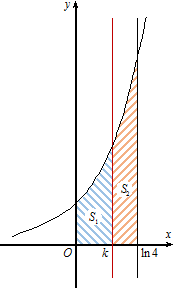
\includegraphics[scale=0.5]{anh27}\hspace*{0.2cm}},{\label{fig:anh27}}]
$y={{e}^{x}}$, $y=0$, $x=0$, $x=\ln 4$. Đường thẳng $x=k\,\,(0<k<\ln 4)$ chia $\left( H \right)$ thành hai phần có diện tích là ${{S}_{1}}$ và ${{S}_{2}}$ như hình vẽ bên. Tìm $k$ để ${{S}_{1}}=2{{S}_{2}}$.
\end{window}\examvspace*{0.cm}
}{\datcot[2]\bonpa
{\sai{$k=\dfrac{2}{3}\ln 4$.}}
{\sai{$k=\ln 2$.}}
{\sai{$k=\ln \dfrac{8}{3}$ }}
{\dung{$k=\ln 3$.}}
\loigiai{Ta có ${{S}_{1}}=\displaystyle\int_{0}^{k}{{{e}^{x}}\text{d}x}=\left. {{e}^{x}} \right|_{0}^{k}={{e}^{k}}-1$ và ${{S}_{2}}=\displaystyle\int_{k}^{\ln 4}{{{e}^{x}}\text{d}x}=\left. {{e}^{x}} \right|_{k}^{\ln 4}=4-{{e}^{k}}$.\\
Ta có ${{S}_{1}}=2{{S}_{2}}\Leftrightarrow {{e}^{k}}-1=2\left( 4-{{e}^{k}} \right)\Leftrightarrow k=\ln 3$. 
}
}
\baitracnghiem{de20170120:b28}{
Ông An có một mảnh vườn hình Elip có độ dài trục lớn
\begin{window}[0,r,{\hspace*{1cm}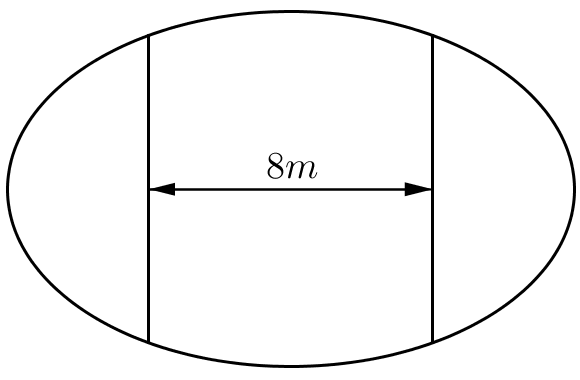
\includegraphics[scale=0.3]{anh28}\hspace*{0.2cm}},{\label{fig:anh28}}]
bằng $16m$ và độ dài trục bé bằng$10m$. Ông muốn trồng hoa trên một dải đất rộng $8m$ và nhận trục bé của elip làm trục đối xứng (như hình vẽ). Biết kinh phí để trồng hoa là $100.000$ đồng/$1\,{{m}^{2}}$. Hỏi ông An cần bao nhiêu tiền để trồng hoa trên dải đất đó? (Số tiền được làm tròn đến hàng nghìn.)
\end{window}\examvspace*{0.cm}
}{\datcot[2]\bonpa
{\sai{$7.862.000$ đồng.}}
{\dung{$7.653.000$ đồng.}}
{\sai{$7.128.000$ đồng.}}
{\sai{$7.826.000$ đồng.}}
\loigiai{Giả sử elip có phương trình $\dfrac{{{x}^{2}}}{{{a}^{2}}}+\dfrac{{{y}^{2}}}{{{b}^{2}}}=1$. \\
Từ giả thiết ta có $2a=16\Rightarrow a=8$ và $2b=10\Rightarrow b=5$ \\
Vậy phương trình của elip là $\dfrac{{{x}^{2}}}{64}+\dfrac{{{y}^{2}}}{25}=1\Rightarrow \left[ \begin{aligned}
  & y=-\frac{5}{8}\sqrt{64-{{y}^{2}}}\,\,\,({{E}_{1}}) \\ 
 & y=\frac{5}{8}\sqrt{64-{{y}^{2}}}\,\,\,({{E}_{1}})  
\end{aligned} \right.$ \\
Khi đó diện tích dải vườn được giới hạn bởi các đường $({{E}_{1}});\,\,({{E}_{2}});\,\,x=-4;\,\,x=4$ và diện tích của dải vườn là $S=2\displaystyle\int_{-4}^{4}{\dfrac{5}{8}\sqrt{64-{{x}^{2}}}\text{d}x}=\dfrac{5}{2}\displaystyle\int_{0}^{4}{\sqrt{64-{{x}^{2}}}\text{d}x}$\\
Tính tích phân này bằng phép đổi biến $x=8\sin t$, ta được $S=80\left( \dfrac{\pi }{6}+\dfrac{\sqrt{3}}{4} \right)$ \\
Khi đó số tiền là $T=80\left( \dfrac{\pi }{6}+\dfrac{\sqrt{3}}{4} \right).100000=7652891,82\simeq 7.653.000$. 
}
}
\baitracnghiem{de20170120:b29}{
Điểm $M$ trong hình vẽ bên là điểm biểu diễn 
\begin{window}[0,r,{\hspace*{1cm}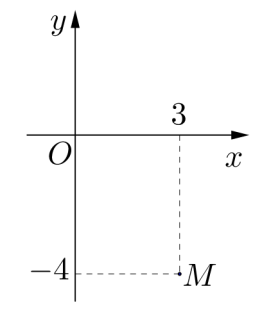
\includegraphics[scale=0.4]{anh29}\hspace*{1cm}},{\label{fig:anh29}}]
 của số phức $z$. Tìm phần thực và phần ảo của số phức $z$.
\end{window}\examvspace*{0.cm}
}{\datcot[4]\bonpa
{\sai{Phần thực là $-4$ và phần ảo là $3$.}}
{\sai{Phần thực là $3$ và phần ảo là $-4i$.}}
{\dung{Phần thực là $3$ và phần ảo là $-4$.}}
{\sai{Phần thực là $-4$và phần ảo là $3i$.}}
\loigiai{Điểm $M$ trong hệ trục $Oxy$ có hoành độ $x=3$ và tung độ $y=-4$.\\ Vậy số phức $z$ có phần thực là $3$ và phần ảo là $-4$. 
}
}
\baitracnghiem{de20170120:b30}{
Tìm số phức liên hợp của số phức $z=i\left( 3i+1 \right)$.
}{\datcot\bonpa
{\sai{$\bar{z}=3-i$.}}
{\sai{$\bar{z}=-3+i$.}}
{\sai{$\bar{z}=3+i$.}}
{\dung{$\bar{z}=-3-i$. }}
\loigiai{Ta có $z=i(3i+1)=3{{i}^{2}}+i=-3+i$, suy ra $\overline{z}=-3-i$. 
}
}
\baitracnghiem{de20170120:b31}{
Tính môđun của số phức $z$ thỏa mãn $z\left( 2-i \right)+13i=1$.
}{\datcot\bonpa
{\dung{$\left| z \right|=\sqrt{34}$.}}
{\sai{$\left| z \right|=34$.}}
{\sai{$\left| z \right|=\dfrac{5\sqrt{34}}{3}$.}}
{\sai{$\left| z \right|=\dfrac{\sqrt{34}}{3}$.}}
\loigiai{$z\left( 2-i \right)+13i=1\Leftrightarrow z=\dfrac{1-13i}{2-i}\Leftrightarrow z=\dfrac{\left( 1-13i \right)\left( 2+i \right)}{\left( 2-i \right)\left( 2+i \right)}\Leftrightarrow z=3-5i$.\\
$\left| z \right|=\sqrt{{{3}^{2}}+{{\left( -5 \right)}^{2}}}=\sqrt{34}.$
}
}
\baitracnghiem{de20170120:b32}{
Kí hiệu ${{z}_{0}}$ là nghiệm phức có phần ảo dương của phương trình $4{{z}^{2}}-16z+17=0$. Trên mặt phẳng tọa độ, điểm nào dưới đây là điểm biểu diễn của số phức $w=i{{z}_{0}}$?
}{\datcot\bonpa
{\sai{${{M}_{1}}\left( \frac{1}{2};2 \right)$.}}
{\dung{${{M}_{2}}\left( -\frac{1}{2};2 \right)$.}}
{\sai{${{M}_{3}}\left( -\frac{1}{4};1 \right)$.}}
{\sai{${{M}_{4}}\left( \frac{1}{4};1 \right)$.}}
\loigiai{Xét phương trình $4{{z}^{2}}-16z+17=0$ có ${\Delta }'=64-4.17=-4={{\left( 2i \right)}^{2}}$.\\
Phương trình có hai nghiệm ${{z}_{1}}=\dfrac{8-2i}{4}=2-\dfrac{1}{2}i,\,\,{{z}_{2}}=\dfrac{8+2i}{4}=2+\dfrac{1}{2}i$.\\
Do ${{z}_{0}}$ là nghiệm phức có phần ảo dương nên ${{z}_{0}}=2+\dfrac{1}{2}i$.
Ta có $w=i{{z}_{0}}=-\dfrac{1}{2}+2i$.\\
Điểm biểu diễn $w=i{{z}_{0}}$ là ${{M}_{2}}\left( -\dfrac{1}{2};2 \right)$.
}
}
\baitracnghiem{de20170120:b33}{
Cho số phức $z=a+bi\,\,\left( a,b\in \mathbb{R} \right)$ thỏa mãn $\left( 1+i \right)z+2\overline{z}=3+2i.$ Tính $P=a+b.$
}{\datcot\bonpa
{\sai{$P=\dfrac{1}{2}.$}}
{\sai{$P=1.$}}
{\dung{$P=-1.$}}
{\sai{$P=-\frac{1}{2}.$}}
\loigiai{$\left( 1+i \right)z+2\overline{z}=3+2i.\left( 1 \right)$. Ta có: $z=a+bi$ $\Rightarrow \overline{z}=a-bi.$\\
Thay vào $\left( 1 \right)$ ta được $\left( 1+i \right)\left( a+bi \right)+2\left( a-bi \right)=3+2i$
$\Leftrightarrow \left( a-b \right)i+\left( 3a-b \right)=3+2i$\\ 
$\Leftrightarrow \left( a-b \right)i+\left( 3a-b \right)=3+2i$
$\Leftrightarrow \left\{ \begin{aligned}
  & a-b=2 \\ 
 & 3a-b=3 \\ 
\end{aligned} \right.\Leftrightarrow \left\{ \begin{aligned}
  & a=\frac{1}{2} \\ 
 & b=-\frac{3}{2}. \\ 
\end{aligned} \right.\Rightarrow P=-1.$
}
}
\baitracnghiem{de20170120:b34}{
Xét số phức $z$ thỏa mãn $\left( 1+2i \right)\left| z \right|=\dfrac{\sqrt{10}}{z}-2+i.$ Mệnh đề nào dưới đây đúng ?
}{\datcot\bonpa
{\sai{$\dfrac{3}{2}<\left| z \right|<2.$}}
{\sai{$\left| z \right|>2.$}}
{\sai{$\left| z \right|<\dfrac{1}{2}.$}}
{\dung{$\dfrac{1}{2}<\left| z \right|<\dfrac{3}{2}.$}}
\loigiai{Ta có ${{z}^{-1}}=\dfrac{1}{{{\left| z \right|}^{2}}}\overline{z}.$ 
Vậy $\left( 1+2i \right)\left| z \right|=\frac{\sqrt{10}}{z}-2+i$$\Leftrightarrow \left( \left| z \right|+2 \right)+\left( 2\left| z \right|-1 \right)i=\left( \frac{\sqrt{10}}{{{\left| z \right|}^{2}}} \right).\overline{z}$\\
$\Rightarrow {{\left( \left| z \right|+2 \right)}^{2}}+{{\left( 2\left| z \right|-1 \right)}^{2}}=\left( \frac{10}{{{\left| z \right|}^{4}}} \right).{{\left| z \right|}^{2}}=\frac{10}{{{\left| z \right|}^{2}}}.$ Đặt ${{\left| z \right|}^{2}}=a>0.$ \\
$\Rightarrow {{\left( a+2 \right)}^{2}}+{{\left( 2a-1 \right)}^{2}}=\left( \frac{10}{{{a}^{2}}} \right)\Leftrightarrow {{a}^{4}}+{{a}^{2}}-2=0\Leftrightarrow \left[ \begin{aligned}
  & {{a}^{2}}=1 \\ 
 & {{a}^{2}}=-2 \\ 
\end{aligned} \right.\Rightarrow a=1\Rightarrow \left| z \right|=1.$
}
}
\baitracnghiem{de20170120:b35}{
Cho hình chóp $S.ABC$ có đáy là tam giác đều cạnh $2a$ và thể tích bằng $+$. Tính chiều cao $h$ của hình chóp đã cho.
}{\datcot\bonpa
{\sai{$h=\dfrac{\sqrt{3}a}{6}$.}}
{\sai{$h=\dfrac{\sqrt{3}a}{2}$.}}
{\sai{$h=\dfrac{\sqrt{3}a}{3}$.}}
{\dung{$h=\sqrt{3}a$.}}
\loigiai{Do đáy là tam giác đều nên ${{S}_{\Delta ABC}}=\frac{{{\left( 2a \right)}^{2}}\sqrt{3}}{4}={{a}^{2}}\sqrt{3}$. \\
Mà $V=\frac{1}{3}{{S}_{\Delta ABC}}.h\Rightarrow h=\frac{3V}{{{S}_{\Delta ABC}}}=\frac{3{{a}^{3}}}{{{a}^{2}}\sqrt{3}}=\sqrt{3}a$. 
}
}
\baitracnghiem{de20170120:b36}{
Hình đa diện nào dưới đây không có tâm đối xứng ?
\begin{center}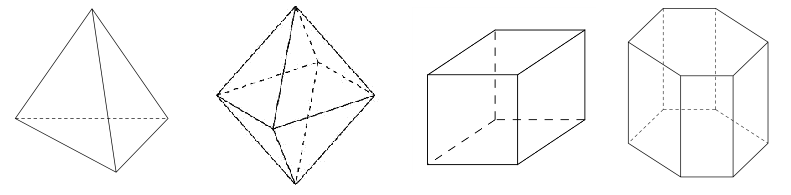
\includegraphics[scale=0.5]{anh36}\end{center}
}{\datcot\bonpa
{\dung{Tứ diện đều.}}
{\sai{Bát diện đều.}}
{\sai{Hình lập phương.}}
{\sai{Lăng trụ lục giác đều.}}
\loigiai{Tứ diện đều làm gì có tâm đối xứng.
}
}
\baitracnghiem{de20170120:b37}{
Cho tứ diện $ABCD$ có thể tích bằng 12 và $G$ là trọng tâm tam giác $BCD$. Tính thể tích $V$ của khối chóp $A.GBC$.
}{\datcot\bonpa
{\sai{$V=3$.}}
{\dung{$V=4$.}}
{\sai{$V=6$.}}
{\sai{$V=5$.}}
\loigiai{$\dfrac{d\left( G,\left( ABC \right) \right)}{d\left( D,\left( ABC \right) \right)}=\dfrac{GI}{DI}=\dfrac{1}{3}\Rightarrow d\left( G,\left( ABC \right) \right)=\dfrac{1}{3}d\left( D,\left( ABC \right) \right)$.\\
Nên ${{V}_{G.ABC}}=\dfrac{1}{3}d\left( G,\left( ABC \right) \right).{{S}_{\Delta ABC}}=\dfrac{1}{3}.{{V}_{DABC}}=4.$  
}
}
\baitracnghiem{de20170120:b38}{
Cho lăng trụ tam giác $ABC.A'B'C'$ có đáy $ABC$ là tam giác vuông cân tại $A$, cạnh $AC=2\sqrt{2}$. Biết $AC'$ tạo với mặt phẳng $\left( ABC \right)$ một góc $60^\circ $ và $AC'=4$. Tính thể tích $V$ của khối đa diện $ABCB'C'$.
A. 	B. 	C. 	D. 

}{\datcot\bonpa
{\sai{$V=\dfrac{8}{3}$.}}
{\sai{$V=\dfrac{16}{3}$.}}
{\sai{$V=\dfrac{8\sqrt{3}}{3}$.}}
{\dung{$V=\dfrac{16\sqrt{3}}{3}$.}}
\loigiai{Tính thể tích của khối đa diện $ABCB'C'$ bằng thể tích khối của lăng trụ $ABC.A'B'C'$ trừ đi thể tích của khối chóp $A.A'B'C'$.
Giả sử đường cao của lăng trụ là $C'H$.\\
Khi đó góc giữa $AC'$ mặt phẳng $\left( ABC \right)$ là góc $\widehat{C'AH}=60^\circ $.\\
Ta có:
$\sin 60{}^\circ =\dfrac{C'H}{AC'}\Rightarrow C'H=2\sqrt{3};{{S}_{\Delta ABC}}=4$\\
$V_{ABC.A'B'C'}=C'H.S_{\Delta ABC}=2\sqrt{3}.\dfrac{1}{2}.\left( 2\sqrt{2} \right)^2=8\sqrt{3}$.\\
$V_{A.A'B'C'}=\dfrac{1}{3}C'H.S_{\Delta ABC}=\dfrac{1}{3}.V_{ABC.A'B'C'}=\dfrac{8\sqrt3}{3}$.\\
$V_{ABB'C'C}=V_{ABC.A'B'C'}-V_{A.A'B'C'}=8\sqrt{3}-\dfrac{8\sqrt{3}}{3}=\dfrac{16\sqrt{3}}{3}$.
}
}
\baitracnghiem{de20170120:b39}{
Cho khối $\left( N \right)$ có bán kính đáy bằng $3$ và diện tích xung quanh bằng $15\pi $. Tính thể tích $V$ của khối nón $\left( N \right)$
}{\datcot\bonpa
{\dung{$V=12\pi $.}}
{\sai{$V=20\pi $.}}
{\sai{$V=36\pi $.}}
{\sai{$V=60\pi $.}}
\loigiai{Gọi $l$ là đường sinh của hình nón, ta có $l=\sqrt{{{R}^{2}}+{{h}^{2}}}$. \\
Diện tích xung quanh của hình nón là $15\pi $, suy ra $15\pi =\pi Rl\Leftrightarrow 15=3.\sqrt{{{3}^{2}}+{{h}^{2}}}\Leftrightarrow h=4$\\
Thể tích khối nón là $V=\frac{1}{3}\pi {{R}^{2}}h=\frac{1}{3}\pi {{.3}^{2}}.4=12\pi $ (đvtt). 
}
}
\baitracnghiem{de20170120:b40}{
Cho hình lăng trụ tam giác đều $ABC.A'B'C'$ có độ dài cạnh đáy bằng $a$ và chiều cao bằng $h$. Tính thể tích $V$ của khối trụ ngoại tiếp lăng trụ đã cho. 
}{\datcot\bonpa
{\sai{$V=\dfrac{\pi {{a}^{2}}h}{9}$.}}
{\dung{$V=\dfrac{\pi {{a}^{2}}h}{3}$.}}
{\sai{$V=3\pi {{a}^{2}}h$.}}
{\sai{$V=\dfrac{\pi {{a}^{2}}h}{9}$.}}
\loigiai{Khối trụ ngoại tiếp lăng trụ tam giác đều có hình tròn đáy là hình tròn ngoại tiếp tam giác đáy của lăng trụ, và chiều cao bằng chiều cao lăng trụ.\\
Tam giác đều cạnh $a$ có bán kính đường tròn ngoại tiếp bằng $\dfrac{\sqrt{3}a}{3}$.\\ Vậy thể tích của khối trụ cần tìm là $V=h.S=h.\pi .{{\left( \dfrac{\sqrt{3}a}{3} \right)}^{2}}=\dfrac{\pi {{a}^{2}}h}{3}$(đvtt). 
}
}
\baitracnghiem{de20170120:b41}{
Cho hình hộp chữ nhật $ABCD.A'B'C'D'$ có $AB=a$, $AD=2a$ và $AA'=2a$. Tính bán kính $R$ của mặt cầu ngoại tiếp tứ diện $ABB'C'$.
}{\datcot\bonpa
{\sai{$R=3a$.}}
{\sai{$R=\dfrac{3a}{4}$.}}
{\dung{$R=\dfrac{3a}{2}$.}}
{\sai{$R=2a$.}}
\loigiai{Ta có $\widehat{AB'C'}=\widehat{ABC'}=90^\circ $ nên mặt cầu ngoại tiếp tứ diện $ABB'C'$ có đường kính $AC'$.\\ Do đó bán kính là $R=\dfrac{1}{2}\sqrt{{{a}^{2}}+{{\left( 2a \right)}^{2}}+{{\left( 2a \right)}^{2}}}=\dfrac{3a}{2}$.
}
}
\baitracnghiem{de20170120:b42}{
Cho hai hình vuông có cùng cạnh bằng 5 
\begin{window}[0,r,{\hspace*{0.1cm}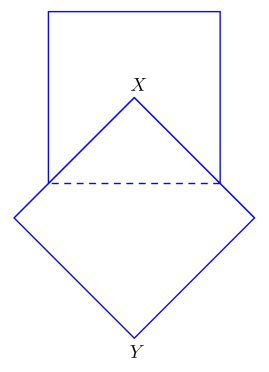
\includegraphics[scale=0.4]{anh42}\hspace*{0.2cm}},{\label{fig:anh42}}]
được xếp chồng lên nhau sao cho đỉnh $X$ của một hình vuông là tâm của hình vuông còn lại (như hình vẽ). Tính thể tích $V$ của vật thể tròn xoay khi quay mô hình trên xung quanh trục $XY$.
\end{window}%\examvspace*{1.5cm}
}{\datcot[2]\bonpa
{\sai{$V=\dfrac{125\left( 1+\sqrt{2} \right)\pi }{6}$.}}
{\sai{$V=\dfrac{125\left( 5+2\sqrt{2} \right)\pi }{12}$.}}
{\dung{$V=\dfrac{125\left( 5+4\sqrt{2} \right)\pi }{24}$.}}
{\sai{$V=\dfrac{125\left( 2+\sqrt{2} \right)\pi }{4}$.}}
\loigiai{Thể tích hình trụ được tạo thành từ hình vuông $ABCD$ là ${{V}_{T}}=\pi {{R}^{2}}h=\dfrac{125\pi }{4}$ \\
Thể tích khối tròn xoay được tạo thành từ hình vuông $XEYF$  là ${{V}_{2N}}=\dfrac{2}{3}\pi {{R}^{2}}h=\dfrac{125\pi \sqrt{2}}{6}$ \\
Thể tích khối tròn xoay được tạo thành từ tam giác  $XDC$  là ${{V}_{{{N}'}}}=\dfrac{1}{3}\pi {{R}^{2}}h=\dfrac{125\pi }{24}$ \\
Thể tích cần tìm $V={{V}_{T}}+{{V}_{2N}}-{{V}_{{{N}'}}}=125\pi \dfrac{5+4\sqrt{2}}{24}$.
}
}
\baitracnghiem{de20170120:b43}{
Trong không gian với hệ tọa độ $Oxyz$, cho hai điểm $A\left( 3;-2;3 \right)$ và $B\left( -1;2;5 \right)$. Tìm tọa độ trung điểm $I$ của đoạn thẳng $AB$.
}{\datcot\bonpa
{\sai{$I\left( -2;2;1 \right)$.}}
{\dung{$I\left( 1;0;4 \right)$.}}
{\sai{$I\left( 2;0;8 \right)$.}}
{\sai{$I\left( 2;-2;-1 \right)$.}}
\loigiai{Tọa độ trung điểm $I$ của đoạn $AB$ với $A(3;-2;3)$ và $B(-1;2;5)$ được tính bởi 
$I\left( 1;\,0;4 \right)$ 
}
}
\baitracnghiem{de20170120:b44}{
Trong không gian với hệ tọa độ $Oxyz$, cho đường thẳng $d:\left\{ \begin{aligned}
  & x=1 \\ 
 & y=2+3t \\ 
 & z=5-t 
\end{aligned} \right.\,\,\left( t\in \mathbb{R} \right)$. Vectơ nào dưới đây là vectơ chỉ phương của $d$ ? 
}{\datcot\bonpa
{\dung{${{\v{u}}_{1}}=\left( 0;3;-1 \right)$.}}
{\sai{${{\v{u}}_{2}}=\left( 1;3;-1 \right)$.}}
{\sai{${{\v{u}}_{3}}=\left( 1;-3;-1 \right)$.}}
{\sai{${{\v{u}}_{4}}=\left( 1;2;5 \right)$.}}
\loigiai{Đường thẳng $d:\left\{ \begin{aligned}
  & x=1 \\ 
 & y=2+3t \\ 
 & z=5-t \\ 
\end{aligned} \right.\ \ (t\in \mathbb{R})$ nhận véctơ $\overrightarrow{u}=(0;3;-1)$ làm VTCP.  
}
}
\baitracnghiem{de20170120:b45}{
Trong không gian với hệ tọa độ $Oxyz$, cho 3 điểm $A\left( 1;0;0 \right)$; $B\left( 0;-2;0 \right)$;$C\left( 0;0;3 \right)$. Phương trình nào dưới dây là phương trình mặt phẳng $\left( ABC \right)$?
}{\datcot\bonpa
{\sai{$\dfrac{x}{3}+\dfrac{y}{-2}+\dfrac{z}{1}=1$.}}
{\sai{$\dfrac{x}{-2}+\dfrac{y}{1}+\dfrac{z}{3}=1$.}}
{\dung{$\dfrac{x}{1}+\dfrac{y}{-2}+\dfrac{z}{3}=1$.}}
{\sai{$\dfrac{x}{3}+\dfrac{y}{1}+\dfrac{z}{-2}=1$.}}
\loigiai{Phương trình mặt phẳng theo đoạn chắn đi qua 3 điểm $A$, $B$,$C$ là: $\dfrac{x}{1}+\dfrac{y}{-2}+\dfrac{z}{3}=1$
}
}
\baitracnghiem{de20170120:b46}{
Trong không gian với hệ tọa độ $Oxyz$, phương trình nào dưới dây là phương trình mặt cầu có tâm $I\left( 1;2;-1 \right)$ và tiếp xúc với mặt phẳng $\left( P \right):x-2y-2z-8=0$?
}{\datcot[2]\bonpa
{\sai{${{\left( x+1 \right)}^{2}}+{{\left( y+2 \right)}^{2}}+{{\left( z-1 \right)}^{2}}=3$.}}
{\sai{${{\left( x-1 \right)}^{2}}+{{\left( y-2 \right)}^{2}}+{{\left( z+1 \right)}^{2}}=3$}}
{\dung{${{\left( x-1 \right)}^{2}}+{{\left( y-2 \right)}^{2}}+{{\left( z+1 \right)}^{2}}=9$.}}
{\sai{${{\left( x+1 \right)}^{2}}+{{\left( y+2 \right)}^{2}}+{{\left( z-1 \right)}^{2}}=9$.}}
\loigiai{Gọi mặt cầu cần tìm là $(S)$.
Ta có $(S)$ là mặt cầu có tâm $I(1;2;-1)$ và bán kính $R$.\\
Vì $(S)$ tiếp xúc với mặt phẳng $(P):x-2y-2z-8=0$ \\ nên ta có
$R=d(I;(P))=\dfrac{\left| 1-2.2-2.(-1)-8 \right|}{\sqrt{{{1}^{2}}+{{(-2)}^{2}}+{{(-2)}^{2}}}}=3$.\\
Vậy phương trình mặt cầu cần tìm là ${{\left( x-1 \right)}^{2}}+{{\left( y-2 \right)}^{2}}+{{\left( z+1 \right)}^{2}}=9$.
}
}
\baitracnghiem{de20170120:b47}{
Trong không gian với hệ tọa độ Oxyz, cho đường thẳng $d:\dfrac{x+1}{1}=\dfrac{y}{-3}=\dfrac{z-5}{-1}$ và mặt phẳng $\left( P \right):3x-3y+2z+6=0$. Mệnh đề nào dưới đây đúng ? 
}{\datcot[2]\bonpa
{\dung{$d$ cắt và không vuông góc với $\left( P \right)$.}}
{\sai{$d$ vuông góc với $\left( P \right)$.}}
{\sai{$d$ song song với $\left( P \right)$.}}
{\sai{$d$ nằm trong $\left( P \right)$.}}
\loigiai{Ta có đường thẳng $d$ đi qua $M\left( -1\text{ ; }0\text{ ; }5 \right)$ có vtcp $\v{u}=\left( 1\,;\,-3\,;\,-1 \right)$ và mặt phẳng $\left( P \right)$ có vtpt $\v{n}=\left( 3\,;\,-3\,;\,2 \right)$
$M\notin \left( P \right)\Rightarrow $ loại đáp án D.\\
$\v{n}\,,\,\v{u}$ không cùng phương $\Rightarrow $ loại đáp án B.\\
$\v{n}\,.\,\v{u}=10$ $\Rightarrow \v{n}\,,\,\v{u}$ không vuông góc $\Rightarrow $ loại đáp án C.
}
}
\baitracnghiem{de20170120:b48}{
Trong không gian với hệ tọa độ Oxyz, cho hai điểm $A\left( -2;3;1 \right)$ và $B\left( 5;\text{ }6;\text{ }2 \right)$. Đường thẳng $AB$cắt mặt phẳng $\left( Oxz \right)$ tại điểm $M$. Tính tỉ số $\dfrac{AM}{BM}$.
}{\datcot\bonpa
{\dung{$\dfrac{AM}{BM}=\dfrac{1}{2}$.}}
{\sai{$\dfrac{AM}{BM}=2$.}}
{\sai{$\dfrac{AM}{BM}=\dfrac{1}{3}$.}}
{\sai{$\dfrac{AM}{BM}=3$.}}
\loigiai{$M\in \left( Oxz \right)\text{ }\Rightarrow M\left( x\text{ ; 0 ; }z \right)$
$\overrightarrow{AB}=\left( 7\text{ ; }3\text{ ; }1 \right)\text{  }\Rightarrow AB=\sqrt[{}]{59}$
$\overrightarrow{AM}=\left( x+2\text{ ;}-3\text{ ; }z-1 \right)$\\ và 
$A,B,M$ thẳng hàng $\Rightarrow \overrightarrow{AM}=k.\overrightarrow{AB}\text{   }\left( k\in \mathbb{R} \right)$ $\Leftrightarrow \left\{ \begin{aligned}
  & x+2=7k \\ 
 & -3=3k \\ 
 & z-1=k \\ 
\end{aligned} \right.\Leftrightarrow \left\{ \begin{aligned}
  & x=-9 \\ 
 & -1=k \\ 
 & z=0 \\ 
\end{aligned} \right.$ $\Rightarrow M\left( -9\text{ ; 0 ; }0 \right)$\\
$\overrightarrow{BM}=\left( -14\text{ ;}-6\text{ ;}-2 \right)\text{  }\Rightarrow BM=\sqrt{118}=2.AB$
}
}
\baitracnghiem{de20170120:b49}{
Trong không gian với hệ tọa độ Oxyz, viết phương trình mặt phẳng $\left( P \right)$ song song và cách đều hai đường thẳng ${{d}_{1}}:\dfrac{x-2}{-1}=\dfrac{y}{1}=\dfrac{z}{1}$ và ${{d}_{2}}:\dfrac{x}{2}=\dfrac{y-1}{-1}=\dfrac{z-2}{-1}$.
}{\datcot[2]\bonpa
{\sai{$\left( P \right):2x-2z+1=0$.}}
{\dung{$\left( P \right):2y-2z+1=0$.}}
{\sai{$\left( P \right):2x-2y+1=0$.}}
{\sai{$\left( P \right):2y-2z-1=0$.}}
\loigiai{${{d}_{1}}$ đi qua điểm $A\left( 2;0;0 \right)$ và có VTCP ${{\v{u}}_{1}}=\left( -1;1;1 \right)$.\\
${{d}_{2}}$ đi qua điểm $B\left( 0;1;2 \right)$ và có VTCP ${{\v{u}}_{2}}=\left( 2;-1;-1 \right)$\\  nên VTPT của $\left( P \right)$ là $\vec{n}=[{{\vec{u}}_{1}},{{\vec{u}}_{2}}]=\left( 0;1;-1 \right)$ 
Khi đó $\left( P \right)$ có dạng $y-z+D=0$ \\
Lại có $\left( P \right)$ cách đều ${{d}_{1}}$ và ${{d}_{2}}$ nên $\left( P \right)$ đi qua trung điểm $M\left( 0;\dfrac{1}{2};1 \right)$ của $AB$
Do đó $\left( P \right):2y-2z+1=0$ 
}
}
\baitracnghiem{de20170120:b50}{
Trong không gian với hệ tọa độ $Oxyz,$ xét các điểm $A\left( 0;0;1 \right)$, $B\left( m;0;0 \right)$, $C\left( 0;n;0 \right)$, $D\left( 1;1;1 \right)$ với $m>0;n>0$ và $m+n=1.$ Biết rằng khi $m$, $n$ thay đổi, tồn tại một mặt cầu cố định tiếp xúc với mặt phẳng $\left( ABC \right)$ và đi qua $d$. Tính bán kính $R$ của mặt cầu đó?
}{\datcot\bonpa
{\dung{$R=1$.}}
{\sai{$R=\dfrac{\sqrt{2}}{2}$.}}
{\sai{$R=\dfrac{3}{2}$.}}
{\sai{$R=\dfrac{\sqrt{3}}{2}$.}}
\loigiai{Gọi $I(1;1;0)$ là hình chiếu vuông góc của $D$ lên mặt phẳng $(Oxy)$\\
Ta có:
Phương trình  của mặt phẳng $(ABC)$ là: $\dfrac{x}{m}+\dfrac{y}{n}+z=1$ \\
Suy ra phương trình tổng quát của $(ABC)$ là $nx+my+mnz-mn=0$\\
Mặt khác $d(I,(ABC))=\dfrac{\left| 1-mn \right|}{\sqrt{{{m}^{2}}+{{n}^{2}}+{{m}^{2}}{{n}^{2}}}}=1$ (vì $m+n=1$) và $ID=1=d(I,(ABC))$ \\
Nên tồn tại mặt cầu tâm $I$ (là hình chiếu vuông góc của $D$ lên mặt phẳng $Oxy$) tiếp xúc với $(ABC)$ và đi qua $D$ 
Khi đó $R=1$
}
}
% \end{document}

\section{Soạn đề bài trực tiếp}
\setcounter{question}{0}
\subsection{Xem đề bài và đáp án}
\begin{verbbox} 
\indebaidapan

\baitracnghiem{abc:b06}{%
Tìm giá trị nhỏ nhất của hàm số $y=\dfrac{x^2+3}{x-1}$ trên đoạn $[2;4]$.
}{
\datcot
\bonpa
{\dung{$\min_{[2;4]} y=6$.}}
{\sai{$\min_{[2;4]} y=-2$.}}
{\sai{$\min_{[2;4]} y=-3$.}}
{\sai {$\min_{[2;4]} y=\dfrac{19}{3}$.}}
\loigiai{
 $y=\dfrac{x^2+3}{x-1}$.\\
$y'=\dfrac{2x(x-1)-x^2-3}{(x-1)^2}=\dfrac{x^2-2x-3}{(x-1)^2}$.\\
$y'=0\Leftrightarrow\left[\begin{matrix}
x=-1\quad \mbox{ loại }\\ 
x=3\quad \mbox{ thỏa mãn }\\ 
\end{matrix}\right.$.\\
Có $y(2)=7; y(3)=6; y(4)=\dfrac{19}{3} \Rightarrow \min\limits_{[2;4]} y=6$.
}
}
\end{verbbox} 
\dkhung

\indebaidapan
\baitracnghiem{abc:b06}{%
Tìm giá trị nhỏ nhất của hàm số $y=\dfrac{x^2+3}{x-1}$ trên đoạn $[2;4]$.
}{
\datcot
\bonpa
{\dung{$\min_{[2;4]} y=6$.}}
{\sai{$\min_{[2;4]} y=-2$.}}
{\sai{$\min_{[2;4]} y=-3$.}}
{\sai {$\min_{[2;4]} y=\dfrac{19}{3}$.}}
\loigiai{
 $y=\dfrac{x^2+3}{x-1}$.\\
$y'=\dfrac{2x(x-1)-x^2-3}{(x-1)^2}=\dfrac{x^2-2x-3}{(x-1)^2}$.\\
$y'=0\Leftrightarrow\left[\begin{matrix}
x=-1\quad \mbox{ loại }\\ 
x=3\quad \mbox{ thỏa mãn }\\ 
\end{matrix}\right.$.\\
Có $y(2)=7; y(3)=6; y(4)=\dfrac{19}{3} \Rightarrow \min\limits_{[2;4]} y=6$.
}
}


\setcounter{question}{0}
\subsection{Xem đề bài, đáp án và lời giải}
\begin{verbbox} 
\indebailoigiai

\baitracnghiem{abc:b06}{%
Tìm giá trị nhỏ nhất của hàm số $y=\dfrac{x^2+3}{x-1}$ trên đoạn $[2;4]$.
}{
\datcot
\bonpa
{\dung{$\min_{[2;4]} y=6$.}}
{\sai{$\min_{[2;4]} y=-2$.}}
{\sai{$\min_{[2;4]} y=-3$.}}
{\sai {$\min_{[2;4]} y=\dfrac{19}{3}$.}}
\loigiai{
 $y=\dfrac{x^2+3}{x-1}$.\\
$y'=\dfrac{2x(x-1)-x^2-3}{(x-1)^2}=\dfrac{x^2-2x-3}{(x-1)^2}$.\\
$y'=0\Leftrightarrow\left[\begin{matrix}
x=-1\quad \mbox{ loại }\\ 
x=3\quad \mbox{ thỏa mãn }\\ 
\end{matrix}\right.$.\\
Có $y(2)=7; y(3)=6; y(4)=\dfrac{19}{3} \Rightarrow \min\limits_{[2;4]} y=6$.
}
}
\end{verbbox} 
\dkhung
\indebailoigiai
\baitracnghiem{abc:b06}{%
Tìm giá trị nhỏ nhất của hàm số $y=\dfrac{x^2+3}{x-1}$ trên đoạn $[2;4]$.
}{
\datcot
\bonpa
{\dung{$\min_{[2;4]} y=6$.}}
{\sai{$\min_{[2;4]} y=-2$.}}
{\sai{$\min_{[2;4]} y=-3$.}}
{\sai {$\min_{[2;4]} y=\dfrac{19}{3}$.}}
\loigiai{
 $y=\dfrac{x^2+3}{x-1}$.\\
$y'=\dfrac{2x(x-1)-x^2-3}{(x-1)^2}=\dfrac{x^2-2x-3}{(x-1)^2}$.\\
$y'=0\Leftrightarrow\left[\begin{matrix}
x=-1\quad \mbox{ loại }\\ 
x=3\quad \mbox{ thỏa mãn }\\ 
\end{matrix}\right.$.\\
Có $y(2)=7; y(3)=6; y(4)=\dfrac{19}{3} \Rightarrow \min\limits_{[2;4]} y=6$.
}
}


\end{document}

